% Artigo para a RBIE sobre o kata. Baseado em rbie_2026_template/main-pt.tex.
% Compilar com: xelatex -shell-escape main && bibtex main && xelatex -shell-escape main (2x)
% Submissão anônima: troque \anonfalse por \anontrue logo abaixo.

\DocumentMetadata{
  lang          = pt-BR,
  pdfversion    = 2.0,
  pdfstandard   = ua-2,
  tagging       = off
}

\documentclass[portuguese]{rbie2026}%

\usepackage[bottom]{footmisc}
\usepackage{tabularray}
\UseTblrLibrary{booktabs}
\usepackage{codehigh}
\usepackage{url}

\clubpenalty  = 100000000
\widowpenalty = 100000000

\newif\ifanon
\anonfalse

% Correção local: \begin{otherlanguage*} da classe imprime a lista de nomes de
% legendas do babel (Bibliografia, Capítulo, Apêndice...) antes do texto dos
% resumos em inglês e espanhol. Aqui só a hifenização é trocada, num grupo local, e só se o padrão do idioma existir.
\makeatletter
\renewenvironment{abstract-es}{%
    \vskip8pt\noindent\keywordfont{\sffamily\textbf{Resumen. }}%
    \begingroup\expandafter\ifx\csname l@\@SBCes\endcsname\relax\else\language=\csname l@\@SBCes\endcsname\fi
}{\endgroup\vskip0pt}
\renewenvironment{abstract-en}{%
    \vskip8pt\noindent\keywordfont{\sffamily\textbf{Abstract. }}%
    \begingroup\expandafter\ifx\csname l@\@SBCen\endcsname\relax\else\language=\csname l@\@SBCen\endcsname\fi
}{\endgroup\vskip0pt}
\makeatother

%----- HEADER INFORMATION. DO NOT EDIT -----------
\jid{RBIE}
\jtitle{Revista Brasileira de Informática na Educação, 20XX, VV:1}
\issn{1414-5685 (print), 2317-6121 (online)}
\doi{10.5753/rbie.yyyy.id}
\copyrightstatement{This work is licensed under a Creative Commons Attribution 4.0 International License}
\jyear{20XX}
\category{Artigo de Pesquisa / Research Paper / Artículo de investigación}
%--------------------------------------------------

\ifanon
\hypersetup{pdftitle={Kata: Ferramenta de Verificação Executável para Apoiar o Ensino de Desenvolvimento de Software com Agentes de Inteligência Artificial},
            pdfauthor={Omitido para revisão}}
\else
\hypersetup{pdftitle={Kata: Ferramenta de Verificação Executável para Apoiar o Ensino de Desenvolvimento de Software com Agentes de Inteligência Artificial},
            pdfauthor={Walter Aoiama Nagai}}
\fi

\title[Kata: ferramenta de verificação executável para apoiar o ensino de software com agentes de IA]{Kata: Ferramenta de Verificação Executável para Apoiar o Ensino de Desenvolvimento de Software com Agentes de Inteligência Artificial}

\engtitle{\textcolor{engtitle}{Kata: Executable Verification Tool to Support the Teaching of Software Development with Artificial Intelligence Agents}}

\thirdlangtitle{\textcolor{thirdlangtitle}{Kata: Herramienta de Verificación Ejecutable para Apoyar la Enseñanza de Desarrollo de Software con Agentes de Inteligencia Artificial}}

\ifanon
\author[Omitido para revisão]{\affil{\textbf{Omitido para revisão}}}
\else
\author[Nagai 2026]{
  \affil{\textbf{Walter Aoiama Nagai} \thinspace \orcidlink{0000-0001-9078-8396} \thinspace \textcolor{blue}{\faEnvelopeO} \enspace [{Universidade Federal de Itajubá} \thinspace | \thinspace \href{mailto:walternagai@unifei.edu.br}{{\textit{walternagai@unifei.edu.br}}}]}
}
\fi

\begin{document}

\begin{frontmatter}
    \maketitle

    \begin{mail}
    \ifanon
      Omitido para revisão.
    \else
      Instituto de Ciências Tecnológicas, Universidade Federal de Itajubá, Itabira, MG, Brasil.
    \fi
    \end{mail}

    \begin{abstract-pt}
        \textit{Introdução.} Agentes de inteligência artificial (IA) escrevem código mais rápido do que qualquer pessoa o revisa, e a supervisão acaba restrita à suíte de testes, que um agente pode satisfazer sem resolver o problema. O mesmo risco existe em disciplinas de programação em que estudantes usam esses agentes. \textit{Métodos.} Este artigo propõe uma ferramenta e um protocolo de estudo. Apresentamos o kata, uma ferramenta de código aberto que conduz uma mudança em cinco domínios (programação, infraestrutura, análise de dados, pesquisa e documentação) por um ciclo de nove fases e a confronta com o repositório por meio de um verificador adversarial (JUDGE), que reexecuta as verificações declaradas e procura oito categorias de fraude. Fundamentamos o ciclo em teoria de ensino, propomos dois casos de uso para um primeiro teste e seis extensões, descrevemos os limites conhecidos do verificador e propomos um protocolo de estudo com estudantes. As regras específicas dos quatro adaptadores de domínio são instruções ao agente e não foram avaliadas. Os dados da verificação técnica, relatados à parte, não são reproduzidos. \textit{Resultados.} A proposta reúne a correspondência entre as fases e os processos cognitivos de Bloom, dois casos de uso para o primeiro teste e seis extensões, cinco desvios do verificador e um protocolo experimental randomizado em grupos paralelos, que prevê cerca de 142 estudantes por grupo. Oito execuções reais, nos cinco domínios, ilustram o ciclo e mostram que o kata executa o que o projeto declara e confere a presença do raciocínio, mas não sua qualidade. \textit{Discussão.} O artigo não mede aprendizagem nem custo de tempo com estudantes. A ferramenta só verifica a presença e a coerência dos registros, e seus desvios conhecidos impedem usá-la como prova única de integridade. O protocolo é o passo seguinte.
    \end{abstract-pt}

    \begin{pchaves}
        Educação em Computação; Agentes de Inteligência Artificial; Verificação de Software; Retorno Formativo; Integridade Acadêmica; Engenharia de Software; Ensino de Software.
    \end{pchaves}

    \begin{abstract-en}
        \textit{Introduction.} Artificial intelligence (AI) agents write code faster than anyone can review it, so oversight collapses onto the test suite, which an agent can satisfy without solving the problem. The same risk exists in programming courses where students use these agents. \textit{Methods.} This article proposes a tool and a study protocol. We present kata, an open-source tool that guides a change in five domains (programming, infrastructure, data analysis, research and documentation) through a nine-phase cycle and confronts it with the repository through an adversarial verifier (JUDGE) that re-runs the declared checks and hunts eight categories of fraud. We ground the cycle in teaching theory, propose two use cases for a first trial and six extensions, describe the verifier's known limits, and propose a study protocol with students. The specific rules of the four domain adapters are instructions to the agent and were not evaluated. The data of the technical verification, reported elsewhere, are not reproduced. \textit{Results.} The proposal comprises the mapping between phases and Bloom's cognitive processes, two use cases for the first trial and six extensions, five verifier bypasses, and a parallel-group randomized experimental protocol that plans about 142 students per group. Eight real runs, in the five domains, illustrate the cycle and show that kata runs what the project declares and checks the presence of reasoning, but not its quality. \textit{Discussion.} The article measures neither learning nor time cost with students. The tool only checks the presence and coherence of records, and its known bypasses prevent its use as sole proof of integrity. The protocol is the next step.
    \end{abstract-en}

    \begin{keywords}
        Computing Education; Artificial Intelligence Agents; Software Verification; Formative Feedback; Academic Integrity; Software Engineering; Software Education.
    \end{keywords}

    \begin{abstract-es}
        \textit{Introducción.} Los agentes de inteligencia artificial (IA) escriben código más rápido de lo que cualquier persona lo revisa, y la supervisión queda limitada a la batería de pruebas, que un agente puede satisfacer sin resolver el problema. El mismo riesgo existe en asignaturas de programación donde el estudiantado usa esos agentes. \textit{Métodos.} Este artículo propone una herramienta y un protocolo de estudio. Presentamos kata, una herramienta de código abierto que conduce un cambio en cinco dominios (programación, infraestructura, análisis de datos, investigación y documentación) por un ciclo de nueve fases y lo confronta con el repositorio mediante un verificador adversarial (JUDGE), que vuelve a ejecutar las verificaciones declaradas y busca ocho categorías de fraude. Fundamentamos el ciclo en teoría de la enseñanza, proponemos dos casos de uso para una primera prueba y seis extensiones, describimos los límites conocidos del verificador y proponemos un protocolo de estudio con estudiantes. Las reglas específicas de los cuatro adaptadores de dominio son instrucciones al agente y no fueron evaluadas. Los datos de la verificación técnica, reportados aparte, no se reproducen. \textit{Resultados.} La propuesta reúne la correspondencia entre las fases y los procesos cognitivos de Bloom, dos casos de uso para la primera prueba y seis extensiones, cinco desvíos del verificador y un protocolo experimental aleatorizado de grupos paralelos, que prevé unos 142 estudiantes por grupo. Ocho ejecuciones reales, en los cinco dominios, ilustran el ciclo y muestran que kata ejecuta lo que el proyecto declara y comprueba la presencia del razonamiento, pero no su calidad. \textit{Discusión.} El artículo no mide el aprendizaje ni el costo de tiempo con estudiantes. La herramienta solo comprueba la presencia y la coherencia de los registros, y sus desvíos conocidos impiden usarla como prueba única de integridad. El protocolo es el paso siguiente.
    \end{abstract-es}

    \begin{pclaves}
        Educación en Computación; Agentes de Inteligencia Artificial; Verificación de Software; Retroalimentación Formativa; Integridad Académica; Ingeniería de Software; Enseñanza de Software.
    \end{pclaves}

    \begin{dates}
        {\sffamily\textbf{Received:}} DD Month YYYY \enspace\textbullet\enspace
        {\sffamily\textbf{Accepted:}} DD Month YYYY \enspace\textbullet\enspace
        {\sffamily\textbf{Published:}} DD Month YYYY
    \end{dates}
\end{frontmatter}


%------------------------------------------
\section{Introdução}
\label{sec:intro}

Agentes de programação baseados em IA generativa já resolvem problemas de programação que se pedem a estudantes. Ao comparar o desempenho de um modelo de código em questões reais de provas de programação introdutória com o de estudantes que as fizeram, \cite{Finnie2022} observaram que o modelo superava a maioria deles. Hoje esses agentes não apenas sugerem trechos: editam arquivos, executam comandos e declaram a tarefa concluída. A Educação em Computação \citep{Bispo2020} precisa decidir o que ensinar e como avaliar diante de modelos que geram código a partir de descrições em linguagem natural, tema de um relatório internacional e de uma síntese recente \citep{Prather2023,Denny2024}. A evidência inicial indica que o efeito da IA generativa sobre iniciantes é desigual. Em um estudo de laboratório, alguns estudantes que não tinham dificuldade aceleraram o trabalho, e nos que tinham, as dificuldades metacognitivas persistiram e a ferramenta pôde agravá-las \citep{Prather2024}.

O ensino de desenvolvimento de software, porém, não se limita a escrever programas. Uma meta-análise sobre o alinhamento entre a formação e a indústria aponta que as maiores lacunas incluem gestão de configuração, processo de software e testes \citep{Garousi2019}. Na nossa leitura, e não na da fonte, essas lacunas se materializam em arquivos de infraestrutura, fluxos de integração, notebooks de dados e documentos, e não só em código de aplicação. Os agentes de código atuam sobre todos esses artefatos. Editam um \textit{Dockerfile}, um \textit{notebook}, um relatório ou uma especificação com a mesma facilidade com que editam um programa, e cada artefato tem a sua forma de ser verificado e a sua forma de ser fraudado. O kata foi desenhado para esse conjunto. Ele tem um ciclo comum de nove fases e cinco domínios (programação, infraestrutura, análise de dados, pesquisa e documentação), que variam o que se deve abrir, observar e vigiar antes de declarar uma tarefa concluída (Seção~\ref{sec:dominios}).

O problema que este artigo trata é anterior à sala de aula e a atravessa. Quando um agente diz ``terminei'', nada executa as verificações que ele afirma ter feito. Ele pode alegar que o código passa na análise estática e nos testes sem que nenhum comando tenha rodado. Pode também ter rodado tudo, mas depois de trocar uma asserção por \texttt{pass}, de modo que o teste passa sem verificar coisa alguma. O \textit{SpecBench}, um \textit{preprint} ainda sem revisão por pares, mede esse fenômeno, conhecido como \textit{reward hacking}. Ele relata que a distância entre os testes visíveis e os testes ocultos cresce 28 pontos percentuais a cada aumento de dez vezes no tamanho do código \citep{SpecBench2026}. É a lei de Goodhart, cujas variantes um \textit{preprint} organiza \citep{Manheim2019}, aplicada ao código: a suíte de testes vira a meta e deixa de ser a medida. Em uma disciplina de programação, o corretor automático de exercícios \citep{Keuning2018} está exposto ao mesmo risco, seja quem o contorna um agente ou uma pessoa.

Duas propostas respondem com disciplina. A primeira é o conjunto das quatro diretrizes que um repositório de terceiros extraiu de observações de Karpathy sobre erros comuns de modelos ao programar: pensar antes de codificar, simplicidade primeiro, mudanças cirúrgicas e execução guiada por objetivos \citep{KarpathySkills2026}. A segunda é o Método Fable, que manda classificar a tarefa antes de agir, exigir evidências e verificar de forma adversarial \citep{Fable2026}. O kata chama de ``Ciclo de Desenvolvimento de Karpathy'' o ciclo que organiza essas diretrizes em fases, e o nome foi dado pelo projeto kata, e não por Karpathy. Ambas as propostas são, porém, texto que instrui, e um modelo pode seguir a instrução, ignorá-la ou segui-la pela metade sem que ninguém perceba a diferença. Modelos de linguagem também não se autocorrigem de forma confiável sem retorno externo \citep{Huang2024}.

Este artigo propõe o \textbf{kata}, uma ferramenta de código aberto que transforma essa disciplina em um ciclo de nove fases, como apoio ao ensino de desenvolvimento de software com agentes de IA. A parte objetiva do ciclo é código Python testado, e não instrução ao modelo. É preciso dizer o que o artigo é. É uma \textbf{proposta de ferramenta e de protocolo de estudo}: descreve a ferramenta e seus limites conhecidos, fundamenta sua adoção em teoria de ensino, propõe casos de uso e um estudo com estudantes. Não avalia efeito sobre a aprendizagem, e nada nele autoriza afirmar que o kata ensina melhor. A verificação técnica da ferramenta, com agentes de IA como sujeitos, é relatada em um manuscrito nosso, separado deste, que não é disponibilizado nesta submissão, e seus dados não são reproduzidos aqui. As questões que guiam a proposta são:

\begin{itemize}
  \item \textbf{QP1.} Que fundamentação pedagógica sustenta o uso do kata no ensino de desenvolvimento de software com agentes de IA, e que evidência cada fase deixa para o retorno formativo?
  \item \textbf{QP2.} Em que situações de ensino de software o kata poderia ser usado, com que fluxo e com que ressalvas, dados os limites conhecidos do verificador?
  \item \textbf{QP3.} Que estudo com estudantes testaria o efeito da ferramenta sobre a aprendizagem?
\end{itemize}

As contribuições são cinco: (i) o kata e a descrição de seus algoritmos objetivos; (ii) uma fundamentação pedagógica do ciclo, apresentada como hipótese de projeto; (iii) dois casos de uso para um primeiro teste em sala e seis extensões, cada um com fluxo, evidência produzida e ressalva; (iv) os limites conhecidos do verificador, reproduzidos e documentados; e (v) um protocolo de estudo com estudantes, ainda não executado. \textbf{O artigo não apresenta dados de estudantes.} As três questões são respondidas por análise conceitual, e os casos de uso e o protocolo são hipóteses a testar.

A Seção~\ref{sec:related-work} posiciona o trabalho. A Seção~\ref{sec:kata} descreve o kata e seus limites conhecidos, e a Seção~\ref{sec:dominios} destaca seus cinco domínios. A Seção~\ref{sec:pedagogia} apresenta a fundamentação pedagógica e a Seção~\ref{sec:casos} os casos de uso. A Seção~\ref{sec:protocolo} propõe o estudo com estudantes, a Seção~\ref{sec:discussao} discute as implicações, a Seção~\ref{sec:limitations} reúne as limitações e a Seção~\ref{sec:conclusion} conclui.


%------------------------------------------
\section{Trabalhos Relacionados}
\label{sec:related-work}

\textbf{Critérios de seleção.} Este artigo não é uma revisão sistemática da literatura inteira. Para a produção nacional, fizemos uma busca sistemática curta em 3 de outubro de 2026 no SOL (SBIE, WEI e EDUCOMP) e na RBIE, com oito \textit{strings} em português para 2022 a 2026. Dos 126 registros obtidos (75 distintos, 52 no período), incluímos 27, por triagem de título e resumo feita por uma única pessoa, com apoio de um assistente de IA e sem concordância entre avaliadores. O protocolo completo está no Apêndice~B, e os registros, a triagem e o código em \texttt{busca/}. Para a literatura internacional, reunimos obras por conhecimento da área e por citação, sem busca sistemática, e priorizamos obras revisadas por pares, marcando as que não são (\textit{preprints} e repositórios) no texto e na lista de referências.

\textbf{IA generativa na Educação em Computação.} Os primeiros trabalhos mediram a capacidade dos modelos em tarefas de disciplinas \citep{Finnie2022} e discutiram oportunidades e desafios da geração automática de código para o ensino \citep{Becker2023}. Um relatório de grupo de trabalho internacional combinou revisão de 71 artigos, um levantamento com estudantes e docentes de 20 países, entrevistas com 22 docentes e orientações éticas \citep{Prather2023}. Uma síntese posterior discute os desafios e as oportunidades que esses modelos trazem a docentes e estudantes \citep{Denny2024}. Entrevistas com 20 docentes de programação introdutória mostram que muitos planejavam, no curto prazo, medidas para coibir a fraude assistida por IA, e que no longo prazo as opiniões divergiam entre proibir as ferramentas e integrá-las às disciplinas \citep{Lau2023}. Há discussões análogas para o ensino de engenharia de software \citep{Daun2023}. Do lado dos estudantes, um experimento controlado com 69 iniciantes (10 a 17 anos) encontrou que o acesso a um gerador de código aumentou o desempenho em tarefas de autoria. O desempenho em tarefas posteriores de modificação manual não diminuiu \citep{Kazemitabaar2023}. Outro, porém, observou iniciantes usando o Copilot e descreveu dificuldades cognitivas e metacognitivas \citep{Prather2023b}, e um terceiro encontrou benefícios e prejuízos distribuídos de forma desigual \citep{Prather2024}. As respostas dos modelos a pedidos de ajuda de iniciantes são em parte úteis e em parte imprecisas \citep{Hellas2023}, o que exige que a pessoa saiba verificar o que recebe. Há também propostas de atividades que treinam a compreensão de código e a formulação de \textit{prompts} \citep{Denny2024b}. Esses trabalhos tratam de como estudantes interagem com a IA. Não tratam de uma ferramenta que verifique, de forma executável, o que foi produzido.

\textbf{Produção nacional.} Dos 27 trabalhos incluídos, 18 tratam de IA generativa no ensino de programação ou de engenharia de software, 4 de correção automática e juízes online, 3 de ensino de teste e 2 de integridade e uso aceitável de IA. Um mapeamento de 52 estudos descreve três papéis da IA generativa no ensino de programação: participante colaborativo, ferramenta de apoio e mediador pedagógico \citep{Bedin2025}. Outro mapeamento, de 18 estudos, trata da programação orientada a objetos \citep{Camilo2026}, e uma revisão examina as estratégias pedagógicas empregadas \citep{Silva2024}. Sobre correção, um estudo mostra que códigos corretos para um corretor automático podem apresentar comportamentos que indicam falhas de aprendizagem \citep{SilvaCaceffo2023}. Outro propõe retorno gerado por modelos de linguagem em lugar de mensagens de erro e resultados de teste \citep{Pimentel2025}. Uma mesa temática propõe discutir como tornar juízes online instrumentos pedagógicos \citep{Delgado2026}. Em teste, estimular estudantes a formular testes melhorou o desempenho deles \citep{Almeida2025}. Sobre integridade, um estudo analisa 1.258 linhas de código do ChatGPT e identifica padrões incomuns em iniciantes \citep{Deus2024}, e uma proposta gradua o uso de IA em cinco níveis \citep{Oliveira2026}. Examinamos o resumo, ou o seu início, de 26 dos 27 trabalhos. O outro não tem resumo e foi triado pelo título. Nenhum descreve um portão que reexecute as verificações declaradas e confronte as afirmações do arquivo de tarefa com o repositório.

\textbf{Avaliação e retorno automáticos.} Uma revisão sistemática de geradores de retorno para exercícios de programação mostra que a maior parte das ferramentas aponta erros e poucas orientam o passo seguinte \citep{Keuning2018}. Avaliar os testes escritos pelos próprios estudantes, e não só o código, é uma estratégia clássica para levá-los da tentativa e erro à reflexão \citep{Edwards2004}. Há também relatos de experiência sobre ensinar a escrever testes, avaliar as suítes dos estudantes, dar incentivo para escrevê-los cedo e sobre os limites da cobertura como critério \citep{Spacco2006}. O risco do outro lado também está documentado: estudantes encontram meios de enganar sistemas de correção automática de exercícios \citep{Kratzke2019}. O retorno formativo tem efeitos substanciais sobre a aprendizagem \citep{Black1998}, e um retorno eficaz responde a três perguntas: aonde vou, como estou indo e o que vem a seguir \citep{Hattie2007}. O andaime (\textit{scaffolding}) é o apoio que permite realizar uma tarefa além da capacidade inicial de quem aprende, ao assumir os elementos que ela ainda não domina \citep{Wood1976}. A literatura posterior destaca que ele deve ser retirado aos poucos. O alinhamento construtivo pede que objetivos, atividades e avaliação se correspondam \citep{Biggs1996}. Um corretor automático é um oráculo de teste, e a literatura de testes de software trata do problema de distinguir o comportamento correto do incorreto \citep{Barr2015}. Deduzimos disso, e não da fonte, que um teste que passa vale o que vale o oráculo por trás dele. Por fim, uma meta-análise aponta lacunas entre o que os cursos de engenharia de software cobrem e o que a indústria espera \citep{Garousi2019}, o que motiva atividades sobre repositórios reais.

\textbf{Verificação de agentes de código.} O \textit{SWE-bench} mede a capacidade de agentes em problemas reais \citep{Jimenez2024}, e o \textit{SpecBench} mede o \textit{reward hacking} \citep{SpecBench2026}. Ambos medem agentes e nenhum entrega um portão que uma equipe ou turma possa rodar nas próprias mudanças. O Método Fable \citep{Fable2026} é o ancestral conceitual mais próximo: define portões de ajuste, de intenção e de verificação adversarial, mas como texto de \textit{prompt}. A avaliação de agentes também precisa considerar o custo, e não só a acurácia, como argumenta um \textit{preprint} \citep{Kapoor2024}.

\textbf{Diferenciação.} O kata difere desses trabalhos em dois pontos. A parte objetiva do portão é código testado, que lê códigos de saída e o estado do Git, e não instrução ao modelo. E o mesmo arquivo de tarefa serve a duas finalidades: sustenta a verificação e deixa um registro por fase que um docente pode ler. Entre os trabalhos que reunimos, nenhum combina as duas coisas nem relata a avaliação de um portão desse tipo. A busca nacional cobriu cinco veículos e \textit{strings} em português, e a internacional não foi sistemática, de modo que a afirmação vale para esse recorte. Por isso o kata é proposto como uma ferramenta a experimentar em sala, e não como solução comprovada.


%------------------------------------------
\section{O Kata}
\label{sec:kata}

O kata (\textit{kata}, ``forma'' ou ``padrão'', como na sequência disciplinada de movimentos das artes marciais) é distribuído no PyPI (\textit{Python Package Index}) como o pacote \texttt{kata-dev}, sob a licença MIT; este artigo descreve a versão 0.8.0 (tag \texttt{v0.8.0}), publicada em outubro de 2026, e indica, onde importa, o que mudou desde a 0.7.2. É um pacote Python de linha de comando com dois \textit{frontends} para agentes (OpenCode e Claude Code), ambos gerados de uma única fonte de fases. A lógica objetiva está sempre no pacote Python, qualquer que seja o \textit{frontend}. Esta seção descreve o projeto do kata e o comportamento que observamos. O artigo não traz evidência independente desse comportamento e não dá acesso ao material da verificação técnica, de modo que o leitor deve lê-la como declaração nossa.

\subsection{O Ciclo de Nove Fases}

A Figura~\ref{fig:ciclo} mostra o ciclo. Uma mudança passa por nove fases: FIT (classificar a tarefa e rotear), THINK (declarar problema, premissas, alternativas e incógnitas antes de codificar), SIMPLIFY (verificar que o código é mínimo), INTENT (comparar o que o código faz, o que o teste espera e o que a especificação diz), SURGICAL (justificar cada arquivo alterado), VERIFY (executar lint, tipos quando declarados, testes e cobertura), TWIN CHECK (procurar o mesmo defeito em outros pontos do projeto), ARTIFACT (conferir as linhas de evidência devidas) e REPORT (relatar o resultado primeiro). Uma fase opcional, o JUDGE, confronta o resultado com o repositório. O modo \texttt{kata -{}-audit} gradua, depois do fato, cada fase de uma tarefa. Na Figura~\ref{fig:ciclo}, observe que só FIT, VERIFY, JUDGE e AUDIT têm borda dupla, ou seja, lógica executável no pacote. As demais fases dependem sobretudo do que a pessoa declara, e é por isso que só as primeiras produzem um veredito ou uma graduação, enquanto as outras produzem registro.

\begin{figure}[t]
    \centering
    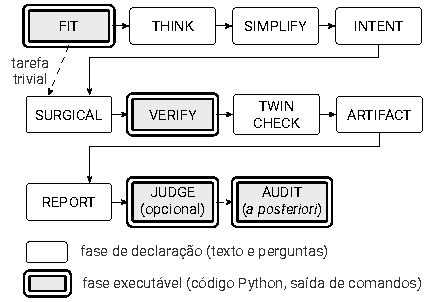
\includegraphics[
      alt={Diagrama de fluxo em três linhas. Na primeira linha, FIT, THINK, SIMPLIFY e INTENT. Na segunda, SURGICAL, VERIFY, TWIN CHECK e ARTIFACT. Na terceira, REPORT, JUDGE (opcional) e AUDIT (a posteriori). Setas ligam as fases na ordem listada, e uma seta tracejada leva de FIT direto a SURGICAL em tarefas triviais. FIT, VERIFY, JUDGE e AUDIT têm borda dupla e fundo cinza, indicando fases executáveis em código Python. As demais têm borda simples, indicando fases de declaração por texto e perguntas.}]{img/fig_ciclo.pdf}
    \caption{O ciclo do kata. As fases de borda dupla têm lógica executável no pacote Python; as demais registram declarações. A seta tracejada é o atalho de tarefas triviais. Diagrama elaborado por nós com o pacote gráfico TikZ do \LaTeX.}
    \label{fig:ciclo}
\end{figure}

A fase FIT mede o \textit{diff} real em relação ao \texttt{HEAD}. Uma tarefa de no máximo um arquivo e menos de dez linhas alteradas é candidata a trivial. Na versão 0.8.0 ainda há uma ressalva: a medida do \textit{diff} inclui os arquivos \texttt{.kata/*.yaml} não rastreados (o próprio arquivo de tarefa e a configuração), de modo que, num projeto que não ignora \texttt{.kata/}, uma mudança de uma linha deixa de ser candidata a trivial. Reproduzimos o caso na 0.8.0 (uma linha alterada: um arquivo; com um \texttt{.kata/x.yaml} não rastreado: dois arquivos e três linhas). O JUDGE e a lista de arquivos do SURGICAL filtram essa escrituração, mas a medida do FIT não a filtra; as demonstrações a escondem porque excluem \texttt{.kata/} do Git. A tarefa só vai direto à verificação, sem o cerimonial de planejamento, se a pessoa confirmar que a mudança não altera comportamento nem exige pesquisa. As demais seguem pelo ciclo completo. A fase VERIFY executa os comandos que o projeto declara em \texttt{.kata/config.yaml} para lint, verificação de tipos (quando declarada), teste e cobertura, ou os padrões Python (\texttt{ruff} e \texttt{pytest}), e julga cada um pelo código de saída, não pelo que o agente afirma. A cobertura só roda se os testes passaram. Na versão 0.8.0, o VERIFY grava no arquivo de tarefa a versão do kata, o gate em vigor, os comandos que rodaram e o horário da execução; o relatório imprime essa evidência e o JUDGE a confronta com a reexecução.


\begin{figure}[t]
    \centering
    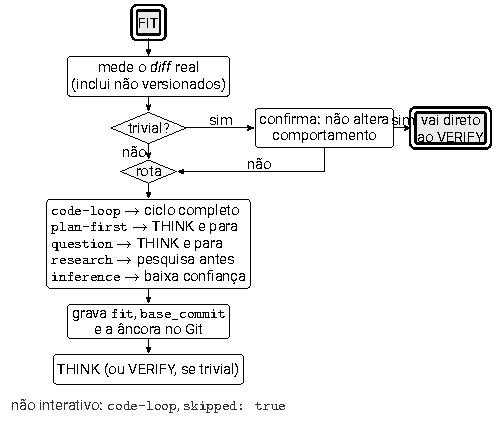
\includegraphics[
      alt={Diagrama de fluxo do FIT. Mede o diff real contra o HEAD, incluindo arquivos não versionados. O losango "trivial?" desvia para a direita: se a pessoa confirma que a mudança não altera comportamento, vai direto ao VERIFY. Caso contrário, o losango "rota" abre cinco caminhos: code-loop leva ao ciclo completo; plan-first e question rodam THINK e param; research pesquisa antes; inference declara baixa confiança. Ao final, grava a classificação, o base_commit e a âncora no Git, e segue para THINK. Uma nota indica que, sem terminal, a rota padrão é code-loop com a fase marcada como pulada.}]{img/fig_fit.pdf}
    \caption{A fase FIT. O diff real é medido incluindo arquivos não versionados; o portão de trivialidade reconfirma com a pessoa, porque "um arquivo, menos de dez linhas" não prova sozinho que o comportamento não mudou; e as cinco rotas divergem. O \texttt{base\_\allowbreak{}commit} e a âncora no Git são gravados aqui.}
    \label{fig:fit}
\end{figure}


\begin{figure}[t]
    \centering
    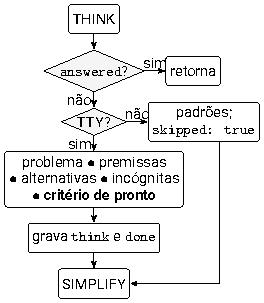
\includegraphics[
      alt={Diagrama de fluxo do THINK. Se a fase já foi respondida, retorna sem reperguntar. Sem terminal, grava padrões e marca a fase como pulada. Em modo interativo, pergunta o problema, as premissas, as alternativas, as incógnitas e o critério de pronto, e grava a seção think e o campo done antes de seguir ao SIMPLIFY.}]{img/fig_think.pdf}
    \caption{A fase THINK. O problema, as premissas, as alternativas, as incógnitas e o \textbf{critério de pronto} são declarados antes de existir evidência. Sem terminal, a seção é gravada como \textit{pulada}, e não como respondida.}
    \label{fig:think}
\end{figure}

\begin{figure}[t]
    \centering
    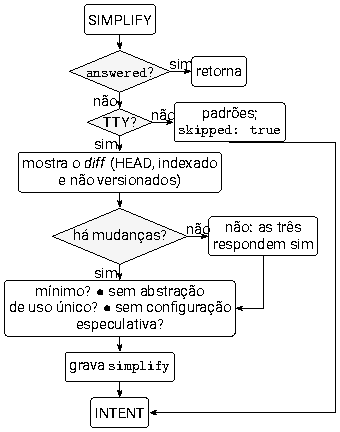
\includegraphics[
      alt={Diagrama de fluxo do SIMPLIFY. Verifica se já foi respondida e se há terminal. Mostra o diff, incluindo arquivos não versionados, e pergunta se há mudanças; sem mudanças, as três respostas são verdadeiras por padrão. As três perguntas são: o código é mínimo, está livre de abstrações de uso único e livre de configuração especulativa.}]{img/fig_simplify.pdf}
    \caption{A fase SIMPLIFY. O \textit{diff}, incluindo os arquivos não versionados que nenhum \texttt{git diff} mostra, é apresentado antes das três perguntas de minimalidade.}
    \label{fig:simplify}
\end{figure}

\begin{figure}[t]
    \centering
    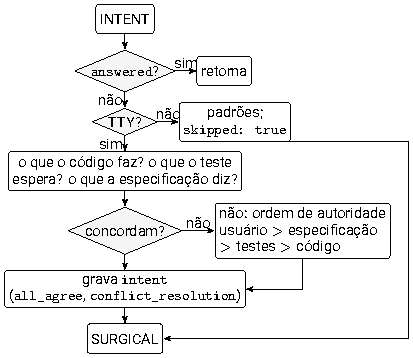
\includegraphics[
      alt={Diagrama de fluxo do INTENT. Compara o que o código faz, o que o teste espera e o que a especificação diz. Se os três discordam, o desacordo é resolvido pela ordem de autoridade: declaração da pessoa, depois especificação, depois testes, depois código. O resultado e a resolução são gravados na seção intent.}]{img/fig_intent.pdf}
    \caption{A fase INTENT. Código, testes e especificação são comparados antes de a mudança acontecer; um desacordo é resolvido pela ordem de autoridade. O JUDGE lê apenas um desacordo \emph{não resolvido} como traição da especificação.}
    \label{fig:intent}
\end{figure}

\begin{figure}[t]
    \centering
    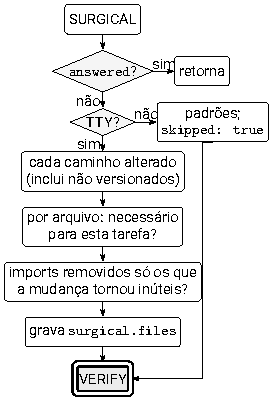
\includegraphics[
      alt={Diagrama de fluxo do SURGICAL. Lista cada caminho alterado, incluindo não versionados, e pergunta por arquivo se ele é necessário para a tarefa; pergunta também se os imports removidos são apenas os que a mudança tornou inúteis. Ao final, grava a lista de arquivos e segue ao VERIFY.}]{img/fig_surgical.pdf}
    \caption{A fase SURGICAL. Cada arquivo alterado é declarado necessário ou não, e essa declaração é o contrato que o JUDGE cobra: arquivo alterado e não declarado é escopo excedente.}
    \label{fig:surgical}
\end{figure}

\begin{figure}[t]
    \centering
    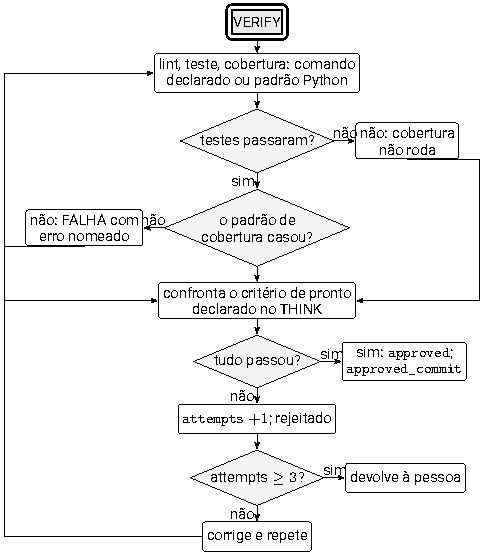
\includegraphics[
      alt={Diagrama de fluxo do VERIFY. Executa lint, teste e cobertura pelo comando declarado ou pelo padrão Python. Se os testes falham, a cobertura não roda. Se o padrão de cobertura não casa, a verificação falha com erro nomeado, em vez de registrar zero por cento como aprovação. Confronta o critério de pronto declarado no THINK. Se tudo passa, grava approved e o approved_commit. Se não, incrementa o contador de tentativas; após três falhas, devolve a tarefa à pessoa; abaixo disso, corrige e repete.}]{img/fig_verify.pdf}
    \caption{A fase VERIFY. Lint, teste e cobertura são julgados pelo código de saída; a cobertura não roda quando os testes falham; um padrão de cobertura que não casa falha com erro nomeado. O contador registra execuções \emph{que falharam}, e após três delas a tarefa é devolvida à pessoa.}
    \label{fig:verify}
\end{figure}

\begin{figure}[t]
    \centering
    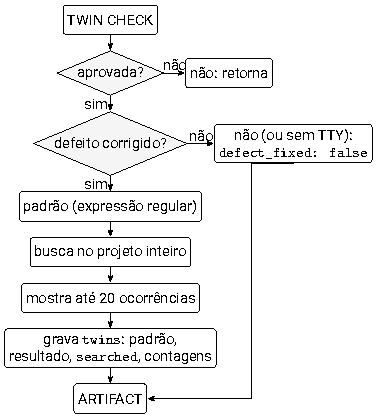
\includegraphics[
      alt={Diagrama de fluxo do TWIN CHECK. Só roda para tarefa aprovada. Pergunta se um defeito foi corrigido; se não, ou sem terminal, grava defect_fixed falso. Se sim, pede um padrão em expressão regular, busca no projeto inteiro, mostra até vinte ocorrências e grava o padrão, o resultado, a marca de busca feita e as contagens.}]{img/fig_twin.pdf}
    \caption{A fase TWIN CHECK. Busca o padrão do defeito corrigido no projeto e registra o resultado, inclusive negativo. Esse registro é o que distingue "não havia defeito" de "ninguém verificou".}
    \label{fig:twin}
\end{figure}

\begin{figure}[t]
    \centering
    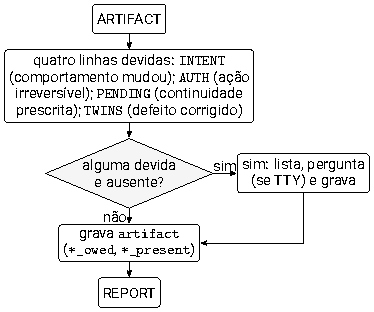
\includegraphics[
      alt={Diagrama de fluxo do ARTIFACT. Verifica quatro linhas devidas: INTENT, quando o comportamento mudou; AUTH, quando houve ação irreversível; PENDING, quando a documentação prescreve continuidade não tomada; e TWINS, quando um defeito foi corrigido. Se alguma linha é devida e está ausente, lista e pergunta; ao final grava os indicadores de devido e presente.}]{img/fig_artifact.pdf}
    \caption{A fase ARTIFACT. Cada uma das quatro linhas de evidência tem seu próprio gatilho; a linha devida e ausente é pedida e registrada. \texttt{TWINS} só é devida quando um defeito foi de fato declarado corrigido.}
    \label{fig:artifact}
\end{figure}

\begin{figure}[t]
    \centering
    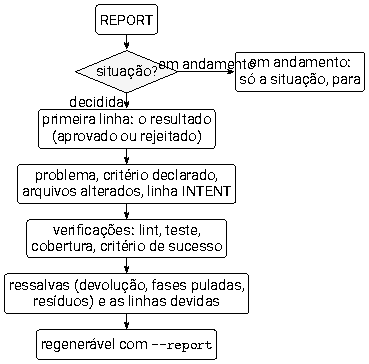
\includegraphics[
      alt={Diagrama de fluxo do REPORT. Se a tarefa está em andamento, imprime só a situação e para. Se está decidida, imprime na primeira linha o resultado, aprovado ou rejeitado; depois o problema, o critério declarado, os arquivos alterados e a linha INTENT; depois as verificações de lint, teste, cobertura e critério de sucesso; depois as ressalvas e as linhas devidas.}]{img/fig_report.pdf}
    \caption{A fase REPORT. O resultado vem primeiro; depois o problema, o critério declarado no THINK, as evidências, as ressalvas e as linhas devidas. Uma tarefa em andamento relata apenas a situação.}
    \label{fig:report}
\end{figure}

\textbf{Arquitetura e garantias do próprio kata.} As fases são escritas uma única vez, em onze arquivos Markdown de origem no tag \texttt{v0.8.0} (dez fases e o orquestrador). Um \textit{script} os expande para cada \textit{frontend}, trocando os nomes das ferramentas por papéis do hospedeiro (executar, ler, perguntar), e um teste falha se os arquivos gerados divergem da origem; 92,8\% das linhas renderizadas são compartilhadas, e o restante é diferença declarada por \textit{frontend}. Quatro adaptadores de domínio (infraestrutura, análise de dados, pesquisa e documentação) estendem o ciclo a tarefas que não são código de aplicação (Seção~\ref{sec:dominios}). O pacote tem portão de cobertura de 70\%, e a integração contínua roda lint, verificação de formato, verificação de divergência das habilidades geradas, testes, o conjunto adversarial e a conferência do pacote construído. Assim, o que se verifica na máquina de quem desenvolve e no servidor não pode divergir.

\subsection{O Verificador Adversarial}

O JUDGE trata o arquivo de tarefa como um conjunto de afirmações, reexecuta as verificações declaradas e compara as afirmações com o \textit{diff} do Git, inclusive com arquivos ainda não versionados. Ele procura oito categorias de fraude. Há testes enfraquecidos (por exemplo, o corpo trocado por \texttt{pass}) e falsa conclusão (o relatório diz que os testes passam e a reexecução falha). Há escopo excedente (o relatório declara um arquivo e a árvore tem quatro), ação não autorizada e traição da especificação (um desacordo de intenção aprovado mesmo assim). Há ainda resíduos, adulteração da linha de base (o \texttt{base\_\allowbreak{}commit} do arquivo diverge da âncora gravada no Git) e trivialidade declarada que o \textit{diff} não sustenta: uma tarefa marcada como trivial com dezenas de arquivos ou centenas de linhas, que o portão de escopo deixaria passar por confiar na própria marca. Os padrões de enfraquecimento cobrem nove famílias de linguagens, e um teste em linguagem não coberta vira uma \textbf{lacuna declarada}, e não um silêncio.

Na versão 0.8.0, o verificador também separa um check que rodou e reprovou de um comando que não pôde rodar: o segundo vira lacuna declarada, e não falsa conclusão, porque transformar ambiente em desonestidade seria um falso positivo. Ele compara a versão do kata, o gate de cobertura e os comandos gravados no arquivo com os da reexecução, e ressalva a diferença em vez de apresentar como equivalente um resultado produzido por outro código ou por outro limiar. E atribui os commits que caem na janela de \textit{diff} aos carimbos das tarefas vizinhas: o trabalho de uma tarefa aprovada e carimbada sai da janela com uma ressalva que nomeia o commit e a tarefa responsáveis; um commit sem carimbo não é atribuído, e o veredito confessa a lacuna em vez de acusar ou absolver.

O veredito é calculado por regras, e não por julgamento do modelo. Qualquer fraude de alta gravidade resulta em \texttt{REFUTED}. Achados de média ou baixa gravidade resultam em \texttt{VERIFIED WITH CAVEATS}. Se não há fraude, mas algo não pôde ser observado, o veredito é \texttt{UNVERIFIABLE}. Um resultado limpo, com todas as reexecuções passando, é \texttt{VERIFIED}. O critério de sucesso do usuário é listado como \textit{aceito sem verificação}, porque nenhum comando o reproduz, e apresentá-lo como verificado seria a fraude que o JUDGE existe para caçar.


\begin{figure}[t]
    \centering
    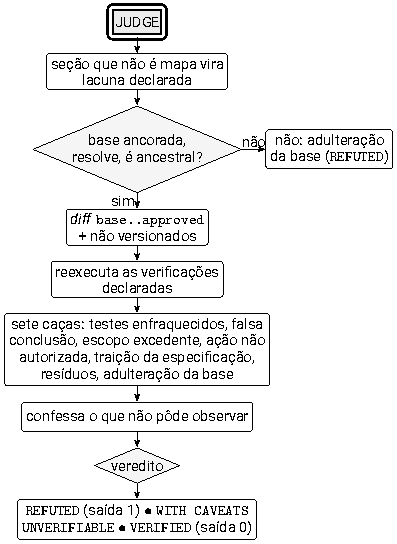
\includegraphics[
      alt={Diagrama de fluxo do JUDGE. Uma seção do arquivo de tarefa que não é mapa vira lacuna declarada. A base é checada: precisa estar ancorada, resolver no histórico e ser ancestral do HEAD; se não, é adulteração da base e o veredito é REFUTED. O diff vai de base até approved, mais os não versionados. Reexecuta as verificações declaradas e roda oito caças: testes enfraquecidos, falsa conclusão, escopo excedente, ação não autorizada, traição da especificação, resíduos, adulteração da base e trivialidade declarada que o diff não sustenta. Confessa o que não pôde observar e calcula o veredito: REFUTED sai com código 1; WITH CAVEATS, UNVERIFIABLE e VERIFIED saem com código 0.}]{img/fig_judge.pdf}
    \caption{A fase JUDGE. O arquivo de tarefa é um conjunto de afirmações; a base é checada de forma adversarial; as verificações declaradas são reexecutadas; oito fraudes são caçadas; e o que não pôde ser observado é confessado.}
    \label{fig:judge}
\end{figure}

\subsection{O Modo de Auditoria}

O \texttt{kata -{}-audit} gradua cada fase em uma de quatro notas. A fase é \textit{seguida} se foi respondida com conteúdo real, \textit{pulada} se foi preenchida com o padrão de uma execução não interativa, sem que ninguém respondesse, \textit{falsificada} se foi marcada como respondida com conteúdo vazio ou padrão (ou se há afirmação de verificação sem evidência) e \textit{degradada} se foi executada sem a habilidade da própria fase carregada. Para cada nota diferente de \textit{seguida}, a ferramenta nomeia o risco concreto criado, como ``as premissas nunca foram declaradas: qualquer solução pode atacar o problema errado''. A graduação é mecânica e cega ao contexto: ela detecta um campo vazio, mas não detecta um campo preenchido com conteúdo plausível e falso.


\begin{figure}[t]
    \centering
    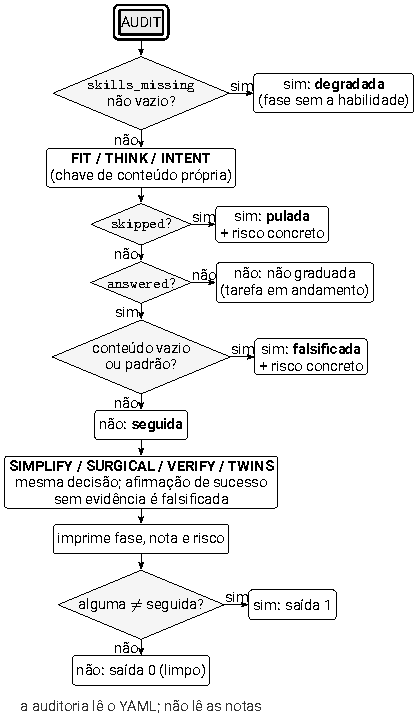
\includegraphics[
      alt={Diagrama de fluxo do AUDIT. Se a lista de habilidades ausentes não está vazia, a fase é graduada como degradada. Para FIT, THINK e INTENT: se pulada, graduada como pulada com o risco concreto; se não respondida, não é graduada; se respondida com conteúdo vazio ou padrão, é falsificada; caso contrário, seguida. SIMPLIFY, SURGICAL, VERIFY e TWINS seguem a mesma decisão, e afirmação de sucesso sem evidência é falsificada. Ao final imprime fase, nota e risco; havendo qualquer nota diferente de seguida, sai com código 1.}]{img/fig_audit.pdf}
    \caption{O modo AUDIT. A auditoria lê o arquivo de tarefa e gradua cada fase como seguida, pulada, falsificada ou degradada, nomeando o risco concreto de cada nota diferente de seguida.}
    \label{fig:audit}
\end{figure}

\subsection{Limites Conhecidos do Verificador}
\label{sec:limites}

O JUDGE é adversarial para as afirmações do arquivo de tarefa, e não para quem controla o repositório. Reproduzimos desvios contra o código do kata, resumidos na Tabela~\ref{tab:desvios}. O mais grave é que um agente que controla o Git pode esvaziar a janela de \textit{diff}, e então um teste esvaziado volta \texttt{VERIFIED}. Alguns caminhos foram estreitados ou fechados na própria 0.8.0, e outros permanecem abertos.

\begin{table*}[ht]
    \centering
    \caption{Desvios do JUDGE reproduzidos contra o código do kata e sua situação no repositório. Código de saída 0 em \texttt{UNVERIFIABLE} é decisão de projeto (falha aberta). Fonte: reprodução nossa em repositório temporário cujo teste foi esvaziado com \texttt{pass}.}
    \label{tab:desvios}
    \begin{tblr}{%
        colspec = {Q[l,m,0.206\linewidth] Q[l,m,0.344\linewidth] Q[l,m,0.258\linewidth]},
        cells   = {font=\small}
        }
        \toprule
        \textbf{Desvio} & \textbf{Efeito observado} & \textbf{Situação} \\
        \midrule
        Reescrever a âncora de base no Git e no YAML & Janela de \textit{diff} vazia; \texttt{VERIFIED} com teste esvaziado & Estreitado (reflog da âncora, \textit{commit} \texttt{3454fc7}); recriá-la ainda escapa localmente; fecha-se em integração contínua com \texttt{-{}-trusted-\allowbreak{}base} \\
        Janela de \textit{diff} vazia (\texttt{approved\_\allowbreak{}commit} igual ao \texttt{base\_\allowbreak{}commit}) & Teste enfraquecido invisível; \texttt{VERIFIED} & Corrigido (\textit{commit} \texttt{3cacc5a}); \texttt{kata -{}-stamp} grava o commit final e fecha a janela depois do \textit{commit} \\
        Fabricar uma lacuna (teste oculto em \texttt{.git/info/exclude} ou em linguagem sem sondas) & \texttt{UNVERIFIABLE} com código 0 passa por quem lê só o código de saída & Aberto; opção de falha fechada é trabalho futuro \\
        Declarar todos os arquivos tocados & Escopo excedente nunca é cobrado, pois \texttt{necessary} é autodeclarado & Aberto \\
        Conteúdo plausível e falso & Auditoria gradua como seguida; resolução de conflito de uma linha desarma a traição da especificação & Aberto \\
        \bottomrule
    \end{tblr}
\end{table*}

Para o uso em sala, a consequência é direta: o JUDGE é um aviso, não uma prova. Um estudante que controla o próprio repositório está na posição do agente da Tabela~\ref{tab:desvios}.

\subsection{Execução 1: o Ciclo Completo}
\label{sec:exemplo}

A Listagem~\ref{lst:exemplo} resume uma execução real do kata sobre um projeto de demonstração: uma calculadora cuja função \texttt{dividir} não trata a divisão por zero. As respostas foram redigidas por nós para a demonstração e não são de estudante. Os ícones do terminal foram trocados por marcadores ASCII.

\begin{listing}[t]
    \caption{Trechos de uma execução real do kata sobre um projeto de demonstração (respostas redigidas por nós; ícones substituídos por marcadores ASCII).}
    \label{lst:exemplo}
\begin{minted}[fontsize=\scriptsize]{text}
$ kata --init dividir-por-zero
  diff: 3 arquivo(s), 16 linha(s) alteradas -> tarefa nao-trivial
  Rota escolhida [1]: 1
  Qual o problema exato que estou resolvendo?
    a função dividir levanta ZeroDivisionError sem guarda
  O que é 'pronto'? o teste test_dividir_por_zero passa
    e a cobertura fica em pelo menos 70%
$ kata --task dividir-por-zero
  O que o código FAZ hoje? dividir levanta ZeroDivisionError
  O que o teste/check ESPERA? o teste espera ValueError
  Código, teste e especificação concordam? [S/n]: n
  [!] Conflito detectado! A ordem de autoridade é:
      declaração do usuário > spec > testes > código
  > python3 -m ruff check src/ tests/        [ok] limpo
  > python3 -m pytest tests/ --tb=short -q   [ok] passou
  > coverage (gate >= 70%)                   [ok] passou (100.0%)
  [!] approved_commit não gravado: o HEAD ainda é o base_commit
      Depois do commit, rode `kata --stamp dividir-por-zero`
  [ok] KATA CYCLE - APROVADO
  TWIN CHECK: padrão 'a / b' encontrado em 1 arquivo(s)
$ kata --audit --task dividir-por-zero
  [ok] FIT, THINK, INTENT, SIMPLIFY, SURGICAL,
       VERIFY, TWINS: followed
\end{minted}
    \vspace{-12pt}
\end{listing}

O FIT mediu o \textit{diff} (três arquivos, 16 linhas) e classificou a tarefa como não trivial. O THINK exigiu problema, premissas, alternativas e critério de pronto antes de qualquer verificação. No INTENT, registramos que o código levanta \texttt{ZeroDivisionError} e o teste espera \texttt{ValueError}. Ao declarar a discordância, o kata exibe a ordem de autoridade entre declaração do usuário, especificação, testes e código, que é o conteúdo conceitual central da fase. O VERIFY executou as verificações declaradas ou os padrões Python e julgou cada uma pelo código de saída. O TWIN CHECK procurou o mesmo padrão no restante do projeto. Na 0.8.0, o relatório imprime também a evidência da execução (gate, comandos e horário) e avisa que o commit final deve ser carimbado com \texttt{kata -{}-stamp}, para fechar a janela do JUDGE.

Duas observações dessa execução importam para a adoção em sala. Na primeira tentativa, o kata rodou com um interpretador Python sem \texttt{ruff} nem \texttt{pytest}. Rejeitou o ciclo com a mensagem de que os módulos não existiam, porque o portão não aprova o que não conseguiu executar (saída reproduzível em \texttt{demos/saidas/01c-sem-\allowbreak{}ferramentas.txt}). Na execução da listagem, porém, o campo de resolução do conflito do INTENT ficou vazio e, mesmo assim, o ciclo foi aprovado. A auditoria graduou todas as fases como seguidas, porque verifica que a fase foi respondida, e não que a resposta é boa. Rodamos o JUDGE sobre essa mesma tarefa (Execução 2, no Apêndice~A), e ele a refutou por traição da especificação.

Sete execuções adicionais estão no Apêndice~A. Nelas, o JUDGE refuta a tarefa acima por traição da especificação e passa a \texttt{VERIFIED} quando o conflito recebe uma frase qualquer (Execução 2). Um teste esvaziado passa em testes e cobertura e só o JUDGE o acusa (Execução 3), e a auditoria acusa as sete fases vazias de um arquivo escrito à mão (Execução 4). Os domínios \texttt{docs}, \texttt{data-analysis}, \texttt{devops} e \texttt{research} são verificados por comandos que o projeto declara, e reprovam, respectivamente, uma flag inexistente, uma remoção de linhas sem registro, uma configuração sem \textit{healthcheck} e um relatório com fonte inexistente (Execuções 5 a 8).

\subsection{O Arquivo de Tarefa}

Cada tarefa vive em \texttt{.kata/<tarefa>.yaml}, um arquivo no formato YAML, de dados legíveis por pessoas. O arquivo é ao mesmo tempo o registro do ciclo e o conjunto de afirmações que o JUDGE confronta com o repositório. As Listagens~\ref{lst:tarefa1} e~\ref{lst:tarefa2} mostram o arquivo completo gerado pelo kata na Execução 1 da Seção~\ref{sec:exemplo}, um projeto de demonstração cujas respostas foram redigidas por nós. Omitimos o bloco \texttt{preflight} (habilidades ausentes) e um bloco de extensão que este artigo não trata. Como o repositório da demonstração não tinha \textit{commits}, faltam os campos \texttt{base\_\allowbreak{}commit} e \texttt{approved\_\allowbreak{}commit}, gravados quando há histórico, e o bloco \texttt{judge}, gravado por \texttt{kata -{}-judge}. A Tabela~\ref{tab:campos} diz, para cada bloco, a que fase pertence, quem o preenche e o que o kata faz com ele. Em uma leitura rápida, os blocos de \texttt{fit} a \texttt{surgical} são declarações da pessoa (ou o padrão de uma execução não interativa). O bloco \texttt{verify} é preenchido pelo kata a partir de códigos de saída, e os blocos \texttt{twins} e \texttt{artifact} são calculados.

\begin{listing}[t]
    \caption{Arquivo de tarefa gerado pelo kata 0.8.0 (parte 1: cabeçalho e fases FIT, THINK, SIMPLIFY e INTENT). Fonte: execução da Seção~\ref{sec:exemplo}; as respostas foram redigidas por nós.}
    \label{lst:tarefa1}
\begin{minted}[fontsize=\scriptsize]{yaml}
schema_version: 1
task: dividir-por-zero
status: approved
domain: coding
done: o teste test_dividir_por_zero passa e a
  cobertura fica em pelo menos 70%
kata_version: 0.8.0
fit:
  trivial: false
  route: code-loop
  reason: corrigir divisão por zero sem guarda
  answered: true
think:
  problem: a função dividir levanta
    ZeroDivisionError sem guarda
  assumptions:
  - a API pública de dividir é estável
  alternatives:
  - guarda com ValueError
  - devolver None
  unknowns: nada
  answered: true
simplify:
  minimum_code: true
  no_single_use_abstractions: true
  no_speculative_config: true
  notes: ''
  answered: true
  skipped: false
intent:
  code_does: dividir levanta ZeroDivisionError
  check_expects: o teste espera ValueError
  spec_says: o README não menciona o caso
  all_agree: false
  conflict_resolution: ''
  answered: true
\end{minted}
    \vspace{-12pt}
\end{listing}

\begin{listing}[t]
    \caption{Arquivo de tarefa (parte 2: fases SURGICAL, VERIFY, AUTH, PENDING, TWIN CHECK e ARTIFACT). Os campos \texttt{skipped} aparecem como \texttt{false} porque as fases foram respondidas.}
    \label{lst:tarefa2}
\begin{minted}[fontsize=\scriptsize]{yaml}
surgical:
  files:
  - path: src/__init__.py
    necessary: true
  - path: src/calculadora.py
    necessary: true
  - path: tests/test_calculadora.py
    necessary: true
  removed_imports_clean: true
  answered: true
  skipped: false
verify:
  ruff_clean: true
  typecheck_clean: null
  tests_pass: true
  coverage_pct: 100.0
  coverage_pass: true
  success_criteria_met: true
  attempts: 0
  hand_back: false
  gate_used: 70.0
  commands:
    lint: python -m ruff check src/ tests/
    test: python -m pytest tests/ --tb=short -q
    coverage: python -m pytest tests/ --cov=src
      --cov-report=term-missing --cov-fail-under=70.0 -q
  ran_at: '2026-10-29T01:58:46+00:00'
auth:
  action_taken: false
  authorized: false
  action: ''
  quote: ''
pending:
  action: ''
  documented: false
twins:
  pattern: a / b
  result: 1 arquivo(s), 1 ocorrência(s)
  searched: true
  defect_fixed: true
  matches_count: 1
  files_count: 1
  fix_applied: false
artifact:
  intent_owed: true
  intent_present: true
  auth_owed: false
  auth_present: false
  pending_owed: false
  pending_present: false
  twins_owed: true
  twins_present: true
\end{minted}
    \vspace{-12pt}
\end{listing}

\begin{table*}[ht]
    \centering
    \caption{Campos do arquivo de tarefa das Listagens~\ref{lst:tarefa1} e~\ref{lst:tarefa2}: fase, quem preenche e o que o kata faz com o bloco. A auditoria gradua um bloco como \textit{falsificado} quando falta o campo-chave indicado ou, em \texttt{verify}, quando há sucesso afirmado sem nenhuma evidência. Fonte: leitura do código do kata 0.8.0 (\texttt{src/kata/cli.py}, \texttt{judge.py} e \texttt{report.py}).}
    \label{tab:campos}
    \begin{tblr}{%
        colspec = {Q[l,m,0.112\linewidth] Q[l,m,0.103\linewidth] Q[l,m,0.172\linewidth] Q[l,m,0.404\linewidth]},
        cells   = {font=\small}
        }
        \toprule
        \textbf{Bloco} & \textbf{Fase} & \textbf{Quem preenche} & \textbf{O que o kata faz com o bloco} \\
        \midrule
        \texttt{task}, \texttt{status}, \texttt{domain} & Geral & O kata & Identifica a tarefa e o domínio; \texttt{status} vira \texttt{approved} ou \texttt{rejected} ao fim do VERIFY \\
        \texttt{kata\_\allowbreak{}version} & Geral & O kata, no VERIFY & Versão que produziu a evidência; o JUDGE a compara com a que está rodando e ressalva a diferença \\
        \texttt{done} & THINK, VERIFY & A pessoa & Critério de pronto declarado antes do código e confrontado com o resultado no VERIFY \\
        \texttt{fit} & FIT & A pessoa & Registra rota e justificativa; \texttt{trivial} parte da medida do \textit{diff} e exige confirmação da pessoa. Auditoria: campo-chave \texttt{reason} \\
        \texttt{think} & THINK & A pessoa & Problema, premissas, alternativas e incógnitas. Auditoria: campo-chave \texttt{problem} \\
        \texttt{simplify} & SIMPLIFY & A pessoa & Três confirmações de minimalidade. Auditoria: campo-chave \texttt{minimum\_\allowbreak{}code} \\
        \texttt{intent} & INTENT & A pessoa & Código, teste e especificação. Com \texttt{all\_\allowbreak{}agree: false} e sem \texttt{conflict\_\allowbreak{}resolution}, o JUDGE aponta traição da especificação (alta gravidade); a resolução é autodeclarada e aceita sem verificação. Auditoria: \texttt{code\_\allowbreak{}does} \\
        \texttt{surgical} & SURGICAL & A pessoa & Lista de arquivos e justificativas. O JUDGE compara a lista com o \textit{diff} real (escopo excedente). Auditoria: \texttt{files} \\
        \texttt{verify} & VERIFY & O kata (e a pessoa, em \texttt{success\_\allowbreak{}criteria\_\allowbreak{}met}) & Resultados de lint, tipos (quando declarados), testes e cobertura vêm de códigos de saída; \texttt{gate\_\allowbreak{}used}, \texttt{commands} e \texttt{ran\_at} registram a evidência da execução. O JUDGE reexecuta e aponta falsa conclusão se divergirem, e ressalva comando, gate ou versão diferentes \\
        \texttt{auth}, \texttt{pending} & ARTIFACT & A pessoa & Ação externa irreversível com a autorização citada (AUTH) e pendência que a documentação prescreve (PENDING) \\
        \texttt{twins} & TWIN CHECK & O kata, a partir da busca & Padrão buscado e ocorrências. Auditoria: falsificado se \texttt{defect\_\allowbreak{}fixed} sem \texttt{searched} \\
        \texttt{artifact} & ARTIFACT & O kata (calculado) & Linhas devidas (\texttt{*\_\allowbreak{}owed}) e presentes (\texttt{*\_\allowbreak{}present}). Se AUTH é devida e falta, o JUDGE aponta ação não autorizada \\
        \texttt{base\_\allowbreak{}commit}, \texttt{approved\_\allowbreak{}commit}, \texttt{judge} & JUDGE & O kata & Não aparecem no exemplo (repositório sem \textit{commits}). Delimitam a janela de \textit{diff} e guardam o veredito; \texttt{kata -{}-stamp} grava o commit final em \texttt{approved\_\allowbreak{}commit} \\
        \bottomrule
    \end{tblr}
\end{table*}

\subsection{Fluxos de Uso no Desenvolvimento de Software}

O kata atende a sete fluxos, todos pela mesma linha de comando. \textit{Antes de um \textit{commit}}: \texttt{kata -{}-init <tarefa>} e \texttt{kata -{}-task <tarefa>} conduzem o ciclo completo. \textit{Planejamento}: \texttt{kata -{}-plan} executa FIT e THINK e para, sem alterar código, e o plano pode ser revisado antes de a primeira linha mudar. \textit{Integração contínua}: \texttt{kata -{}-check-only} roda lint, testes e cobertura de forma não interativa e sai com código 1 se algo falha. \textit{Revisão antes de integrar}: \texttt{kata -{}-task <tarefa> -{}-judge} reexecuta as verificações e caça fraudes e, em integração contínua, \texttt{-{}-trusted-base <ref>} toma o piso do \textit{diff} de uma referência que o agente não controla. \textit{Fechamento}: depois do \textit{commit}, \texttt{kata -{}-stamp <tarefa>} grava o commit que encerra o trabalho em \texttt{approved\_\allowbreak{}commit}, fechando a janela do JUDGE; sem ele, a próxima tarefa contamina a janela desta. \textit{Auditoria}: \texttt{kata -{}-audit} gradua as fases de uma tarefa já concluída. \textit{Instalação}: \texttt{kata -{}-install} copia as habilidades empacotadas para o diretório de configuração do hospedeiro, e \texttt{kata -{}-doctor} confere se estão completas e se a versão que as gravou é a do \texttt{kata} que está rodando. Cada projeto declara em \texttt{.kata/config.yaml} os próprios comandos de lint, tipos, teste e cobertura, o que permite usar o kata fora de Python; uma chave desconhecida ou um operador de \textit{shell} no comando viram erro nomeado, e não um padrão silencioso. Em uma disciplina, os fluxos de integração contínua e de revisão são as formas naturais de conferir entregas. Os de ciclo e auditoria servem para acompanhar o processo.

%------------------------------------------
\section{Os Domínios do Kata}
\label{sec:dominios}

O ciclo da Seção~\ref{sec:kata} é o mesmo em todo o kata, mas o que significa abrir a evidência, observar o resultado e desconfiar de uma afirmação muda conforme o artefato. Por isso o kata tem um domínio padrão, \texttt{coding}, e quatro adaptadores de domínio, \texttt{devops}, \texttt{data-analysis}, \texttt{research} e \texttt{docs}. O arquivo de tarefa declara o domínio no campo \texttt{domain}, que vale \texttt{coding} quando omitido. Para os outros, a instrução do orquestrador manda o agente carregar o adaptador \texttt{kata-<domínio>} logo depois do FIT. Os adaptadores são opcionais: se o agente não consegue carregá-lo, a instrução manda registrar a falta em \texttt{preflight.skills\_\allowbreak{}missing}, e a auditoria, ao ler esse registro, marca uma entrada \texttt{preflight} como degradada. Quem escreve o registro é o agente, e nada impede que o omita. Um nome de domínio desconhecido gera um aviso do pacote, e o ciclo segue como \texttt{coding}. As Tabelas~\ref{tab:dominios} e~\ref{tab:dominios-b} comparam os cinco domínios.

\begin{table*}[ht]
    \centering
    \caption{Os cinco domínios do kata, parte 1: artefatos, evidência a abrir antes de agir e ordem de autoridade. A coluna de autoridade mostra a ordem que vale depois da declaração explícita do usuário, que é sempre a maior. Fonte: leitura dos adaptadores em \texttt{domains/} e do código do kata 0.8.0.}
    \label{tab:dominios}
    \begin{tblr}{%
        colspec = {Q[l,m,0.34\linewidth] Q[l,m,0.28\linewidth] Q[l,m,0.24\linewidth]},
        cells   = {font=\small}
        }
        \toprule
        \textbf{Domínio e artefatos} & \textbf{Evidência a abrir antes de agir} & \textbf{Autoridade (após o usuário)} \\
        \midrule
        \texttt{coding}: código de aplicação e testes & Diff, testes e especificação & Especificação, testes, código (fase INTENT) \\
        \texttt{devops}: Docker e Compose, Terraform, Nginx, CI/CD, \textit{deploy}, \textit{healthchecks} & Arquivos de configuração, documentação operacional e estado do ambiente & Documentação operacional, configuração versionada, estado observado \\
        \texttt{data-analysis}: pandas, Polars, SQL, \textit{notebooks}, painéis, \textit{pipelines} & Scripts, esquema dos dados e dicionário de dados & Dicionário de dados, código de análise, dados observados \\
        \texttt{research}: APIs, bibliotecas, literatura, comparações, experimentos & Fontes primárias e código observado & Fonte primária, código observado \\
        \texttt{docs}: README, guias, \textit{changelog}, docstrings, especificações & Documentos vizinhos e a fonte técnica que descrevem & Fonte técnica real, convenções do repositório \\
        \bottomrule
    \end{tblr}
\end{table*}

\begin{table*}[ht]
    \centering
    \caption{Os cinco domínios do kata, parte 2: verificação por observação e fraudes que cada adaptador manda o agente e o revisor procurarem. Esses tipos de fraude são instruções dos adaptadores, e não código do JUDGE. Fonte: leitura dos adaptadores em \texttt{domains/} e do código do kata 0.8.0.}
    \label{tab:dominios-b}
    \begin{tblr}{%
        colspec = {Q[l,m,0.17\linewidth] Q[l,m,0.34\linewidth] Q[l,m,0.34\linewidth]},
        cells   = {font=\small}
        }
        \toprule
        \textbf{Domínio} & \textbf{Verificação por observação} & \textbf{Fraudes que o adaptador manda caçar} \\
        \midrule
        \texttt{coding} & Lint, testes e cobertura, por \texttt{ruff} e \texttt{pytest} ou pelos comandos do projeto & As oito categorias do JUDGE (Seção~\ref{sec:kata}) \\
        \texttt{devops} & \texttt{docker compose config} e \texttt{ps}; \texttt{docker build}; \texttt{nginx -t} e \textit{curl} no \textit{healthcheck}; sintaxe do \textit{workflow} & \texttt{unverified\_\allowbreak{}deploy}, \texttt{weakened\_\allowbreak{}healthcheck}, \texttt{secret\_\allowbreak{}in\_\allowbreak{}diff}, \texttt{unpinned\_\allowbreak{}image}, \texttt{missing\_\allowbreak{}volume\_\allowbreak{}port}, \texttt{silent\_\allowbreak{}config}, \texttt{unauthorized\_\allowbreak{}action}, \texttt{prod\_\allowbreak{}direct\_\allowbreak{}edit} \\
        \texttt{data-analysis} & Executar o script ou \textit{notebook} com saída 0; \texttt{EXPLAIN} em amostra; conferir forma e nulos; renderizar o gráfico & \texttt{unverified\_\allowbreak{}analysis}, \texttt{cherry\_\allowbreak{}picking}, \texttt{data\_\allowbreak{}leak}, \texttt{unpinned\_\allowbreak{}dependency}, \texttt{silent\_\allowbreak{}drop}, \texttt{fabricated\_\allowbreak{}number}, \texttt{unauthorized\_\allowbreak{}access} \\
        \texttt{research} & Abrir o trecho da fonte; reproduzir com \textit{script} mínimo; apontar arquivo e linha; separar observado de inferido & \texttt{fabricated\_\allowbreak{}source}, \texttt{hallucinated\_\allowbreak{}behavior}, \texttt{cherry\_\allowbreak{}picking\_\allowbreak{}sources}, \texttt{stale\_\allowbreak{}source}, \texttt{unverifiable\_\allowbreak{}claim} \\
        \texttt{docs} & Rodar o comando citado; buscar a \textit{flag} na fonte; derivar contagens da implementação & \texttt{drift\_\allowbreak{}numerico}, \texttt{fabricated\_\allowbreak{}command}, \texttt{stale\_\allowbreak{}procedure}, \texttt{orphan\_\allowbreak{}section} \\
        \bottomrule
    \end{tblr}
\end{table*}

\textbf{O que é executável e o que é instrução.} Os tipos de fraude da última coluna da Tabela~\ref{tab:dominios-b} são instruções escritas nos adaptadores, e não lógica do JUDGE. Dos 24 tipos listados, só \texttt{unauthorized\_\allowbreak{}action} aparece no pacote Python, porque coincide com uma das oito categorias do JUDGE, e os outros 23 não existem no código. O pacote só usa o campo \texttt{domain} para imprimir o domínio e avisar de um adaptador desconhecido. O JUDGE continua a procurar as oito categorias de fraude, em qualquer domínio. Fora de \texttt{coding}, a parte executável da verificação vem dos comandos que o projeto declara em \texttt{.kata/config.yaml}, que o kata roda como foram escritos e julga pelo código de saída. Uma atividade de infraestrutura poderia declarar \texttt{docker compose config} como verificação, e uma de dados, a execução do \textit{notebook}. As Execuções 5 a 8 do Apêndice~A fazem isso para os domínios \texttt{docs}, \texttt{data-analysis}, \texttt{devops} e \texttt{research}, com comandos próprios. Sem essa declaração, vale o padrão Python, que não faz sentido para esses artefatos. Daí uma consequência para o ensino: nesses domínios a vigilância contra fraudes específicas, como o número inventado em um relatório ou a fonte inexistente, depende do agente e do docente, e não de uma checagem automática.

Todos os adaptadores compartilham três contratos. O primeiro é a ordem de autoridade, em que a inferência do modelo só vale como baixa confiança e o conflito entre documento e artefato é resolvido perguntando ao usuário. O segundo é a verificação por observação: uma afirmação só vale se for observada, de modo que ``fiz o \textit{deploy}'' sem \texttt{docker compose ps} é uma afirmação não verificada. O terceiro são as linhas vermelhas, ações que exigem uma intervenção humana documentada. São exemplos publicar dados pessoais, executar \textit{deploy} ou \textit{push} sem a linha AUTH com a citação do usuário, pôr segredos no \textit{diff} ou no arquivo de tarefa e afirmar um fato de API sem abrir a fonte.

\subsection{Contexto de Ensino por Domínio}

Os usos a seguir são hipóteses, derivadas dos adaptadores e da Seção~\ref{sec:pedagogia}.

\textbf{Programação (\texttt{coding}).} É o domínio dos casos 1 a 7 da Seção~\ref{sec:casos}: disciplinas de programação, testes, manutenção e projeto, em que o objeto é código e o resultado é verificado por testes.

\textbf{Infraestrutura (\texttt{devops}).} Disciplinas de redes, sistemas, implantação ou DevOps, em que o estudante configura contêineres, servidor web ou fluxos de integração. A verificação por observação ensina uma disciplina de trabalho (\textit{só afirmar o que se observou}), e as linhas vermelhas sobre segredos e ações irreversíveis correspondem a conteúdos de segurança. Ressalvas: exige Docker no laboratório, e o JUDGE só confere o que o projeto declarar como verificação.

\textbf{Análise de dados (\texttt{data-analysis}).} Disciplinas de ciência de dados, estatística aplicada ou \textit{business intelligence}, com \textit{notebooks} e consultas. Os tipos de fraude do adaptador (seleção conveniente de amostra, número sem fonte, remoção silenciosa de linhas) descrevem riscos reais em relatórios de estudantes. Ressalvas: nenhum desses riscos é detectado por código, e dados pessoais exigem o tratamento da Seção~\ref{sec:casos} e da LGPD.

\textbf{Pesquisa (\texttt{research}).} Metodologia científica, iniciação científica e trabalhos de conclusão, em que o estudante investiga uma biblioteca, compara alternativas ou revisa literatura. A exigência de fonte primária e a separação entre o observado e o inferido se aplicam a um risco que o adaptador trata: a invenção de fontes e comportamentos. Ressalvas: o adaptador pede que o agente cite o trecho da fonte, mas quem confere a citação é o docente.

\textbf{Documentação (\texttt{docs}).} Redação técnica, engenharia de requisitos e documentação de projeto, com especificações e registros de decisão. A regra de que todo comando, \textit{flag} ou contagem citada tem fonte no código e a de que, havendo divergência, é o documento que se corrige treinam a detecção de documentação desatualizada. Ressalvas: a verificação roda o comando citado, o que só funciona para documentos técnicos de software.

%------------------------------------------
\section{Fundamentação Pedagógica da Proposta}
\label{sec:pedagogia}

Esta seção responde à QP1 por análise conceitual. A correspondência que propomos é uma hipótese de projeto nossa, e nenhuma parte dela foi validada com estudantes ou docentes.

\textbf{O ciclo como andaime.} O andaime sustenta uma atividade que a pessoa ainda não executa sozinha, ao assumir os elementos da tarefa que ela ainda não domina \citep{Wood1976}, e deve ser retirado aos poucos, como a literatura posterior destaca. O ciclo fixa a ordem do trabalho disciplinado: declarar antes de codificar, justificar cada arquivo, verificar com comandos reais. Quem está começando pode não ter o hábito dessas etapas, e o ciclo as torna explícitas. A retirada gradual do andaime é uma decisão de política da disciplina, e o kata não a automatiza (Seção~\ref{sec:casos}, caso 7).

\textbf{Fases e dificuldades de iniciantes.} Em um estudo de laboratório com iniciantes que programavam com IA generativa, \cite{Prather2024} descrevem dificuldades metacognitivas conhecidas, como formar um modelo conceitual incorreto do problema e ter uma falsa sensação de progresso depois de testar a solução. Os autores propõem andaimar a experiência com a ferramenta. Lemos o ciclo como uma resposta possível, e isso é uma hipótese. A fase THINK pede o problema, as premissas e o critério de pronto antes do código, o que expõe o modelo conceitual da pessoa. A fase VERIFY confronta a sensação de progresso com códigos de saída. A fase INTENT obriga a pôr lado a lado o que o código faz, o que o teste espera e o que a especificação diz.

\textbf{Reflexão na ação e testes.} \cite{Edwards2004} argumenta que o teste de software promove a formação de hipóteses e a validação experimental, centrais à reflexão na ação. Segundo ele, avaliar a capacidade de demonstrar a correção por testes reforça essas habilidades. Em termos do kata, as premissas do THINK fazem o papel de hipóteses e o VERIFY, o de validação experimental, e o JUDGE cobra que o experimento não tenha sido esvaziado. Esta também é uma hipótese de leitura, e não um resultado.

\textbf{O arquivo e a auditoria como retorno formativo.} O retorno é formativo quando informa a pessoa sobre a distância entre o desempenho atual e o desejado, a tempo de ela agir \citep{Black1998}. Um retorno eficaz responde a três perguntas: aonde vou, como estou indo e o que vem a seguir \citep{Hattie2007}. Cada fase deixa um registro que o docente pode ler sem reconstruir o raciocínio do estudante. As notas de auditoria apontam fases omitidas ou vazias e dizem qual risco isso criou, o que é retorno sobre o processo, e não apenas sobre o resultado.

\textbf{Mapeamento para objetivos de aprendizagem.} A Tabela~\ref{tab:bloom} relaciona cada fase ao processo cognitivo dominante na taxonomia revisada de Bloom \citep{Anderson2001}, à evidência que a fase deixa e ao que o pacote verifica automaticamente. Observe a última coluna: nas fases de declaração (THINK, SIMPLIFY), o pacote só verifica que o campo foi preenchido, e nada verifica que a declaração é boa. Por isso, o retorno automático cobre a presença do raciocínio e a conferência dos fatos (o que os comandos retornaram, quais arquivos mudaram), mas não a qualidade do julgamento. Essa parte continua sendo trabalho de docentes e de colegas.

\begin{table*}[ht]
    \centering
    \caption{Leitura pedagógica das fases do kata. Os processos cognitivos (Lembrar, Compreender, Aplicar, Analisar, Avaliar e Criar) seguem a taxonomia revisada de Bloom \citep{Anderson2001}; a atribuição a cada fase é interpretação nossa. N/A: nenhuma verificação automática além da presença do campo. Fonte: nossa análise do código do kata 0.8.0.}
    \label{tab:bloom}
    \begin{tblr}{%
        colspec = {Q[l,m,0.103\linewidth] Q[l,m,0.146\linewidth] Q[l,m,0.275\linewidth] Q[l,m,0.275\linewidth]},
        cells   = {font=\small}
        }
        \toprule
        \textbf{Fase} & \textbf{Processo cognitivo} & \textbf{Evidência que a fase deixa} & \textbf{Verificação automática} \\
        \midrule
        FIT & Analisar & Classificação da tarefa e rota escolhida & Diff medido (arquivos e linhas); atalho para tarefas triviais \\
        THINK & Compreender, Analisar & Problema, premissas, alternativas, incógnitas e critério de pronto & N/A \\
        SIMPLIFY & Avaliar & Confirmação de código mínimo, sem abstração especulativa & N/A \\
        INTENT & Analisar, Avaliar & O que o código faz, o que o teste espera e o que a especificação diz & Desacordo não resolvido é fraude de alta gravidade no JUDGE \\
        SURGICAL & Avaliar & Arquivos alterados, cada um justificado & Comparação com o diff real (escopo excedente) \\
        VERIFY & Aplicar, Avaliar & Resultados de lint, testes e cobertura & Comandos executados e códigos de saída \\
        TWIN CHECK & Aplicar, Analisar & Padrão do defeito e ocorrências encontradas & Busca textual no projeto \\
        ARTIFACT, REPORT & Avaliar, Criar & Linhas devidas e relatório com o resultado primeiro & Presença das linhas devidas \\
        JUDGE & Avaliar (autocrítica) & Veredito e fraudes encontradas & Reexecução e comparação com o Git \\
        \bottomrule
    \end{tblr}
\end{table*}

\textbf{Da nota de auditoria à pergunta formativa.} Cada nota diferente de \textit{seguida} vem com o risco que a omissão cria, e esse texto pode orientar a conversa entre docente e estudante. A Tabela~\ref{tab:rubrica} reproduz as mensagens de risco da ferramenta (nas palavras do código) e sugere, para cada fase, uma pergunta que o docente poderia fazer. As perguntas são sugestões nossas e não foram testadas em sala. A ideia é que a auditoria aponte \textit{onde} olhar, e a pergunta abra a conversa sobre \textit{por quê}, o que corresponde à pergunta ``como estou indo'' do modelo de \cite{Hattie2007}.

\begin{table*}[ht]
    \centering
    \caption{Do risco nomeado pela auditoria a uma pergunta formativa. A coluna central reproduz as mensagens do kata 0.8.0 (\texttt{\_\allowbreak{}AUDIT\_\allowbreak{}RISKS}, \texttt{src/kata/report.py}), traduzidas para o texto corrido e com ``spec'' escrito por extenso; a coluna da direita é sugestão nossa, não validada.}
    \label{tab:rubrica}
    \begin{tblr}{%
        colspec = {Q[l,m,0.086\linewidth] Q[l,m,0.387\linewidth] Q[l,m,0.318\linewidth]},
        cells   = {font=\small}
        }
        \toprule
        \textbf{Fase} & \textbf{Risco que o kata nomeia} & \textbf{Pergunta formativa sugerida} \\
        \midrule
        FIT & rota e trivialidade não classificadas por humano: esforço pode ser desperdiçado em tarefa trivial ou mal roteada & Por que esta tarefa é, ou não é, trivial? O que mudaria sua escolha de rota? \\
        THINK & \textit{assumptions} nunca declaradas: qualquer solução pode atacar o problema errado & Qual premissa, se falsa, derrubaria sua solução? Como você a testaria? \\
        SIMPLIFY & minimalidade afirmada sem ninguém confrontar o \textit{diff} com o pedido: abstrações especulativas podem passar sem revisão & Que parte da mudança você removeria sem deixar de atender ao pedido? \\
        SURGICAL & cada arquivo declarado necessário sem ninguém conferir: escopo extra pode entrar sem ser notado & Qual arquivo você tocou que o pedido não exige? \\
        INTENT & código, teste e especificação podem discordar sem registro: comportamento muda sem intenção verificada & Quando código e teste discordam, quem tem razão, e por quê? \\
        VERIFY & sucesso afirmado sem evidência de execução: a tarefa pode estar aprovada sobre nada & O que a saída deste comando prova, e o que ela não prova? \\
        TWINS & defeito corrigido sem busca de recorrência: o mesmo padrão pode se repetir em outros lugares & Onde mais este mesmo erro poderia estar? \\
        \bottomrule
    \end{tblr}
\end{table*}

\textbf{Alinhamento construtivo.} O alinhamento construtivo \citep{Biggs1996} pede que o docente parta dos resultados de aprendizagem desejados e escolha atividades e avaliação que os evidenciem. Aqui, a Tabela~\ref{tab:bloom} permite fazer o caminho inverso a partir de uma fase. Se o resultado desejado é que a pessoa saiba justificar o escopo de uma mudança, a fase SURGICAL é a atividade e o arquivo de tarefa, a evidência. Fases que não correspondem a nenhum resultado da disciplina podem ser dispensadas por política da disciplina (Seção~\ref{sec:casos}, caso 7).

\textbf{Riscos pedagógicos da própria ferramenta.} A proposta tem riscos que o docente precisa vigiar. O primeiro é o ritual: a pessoa pode preencher os campos para cumprir a exigência, e a Execução 1 mostra que a auditoria graduaria como seguido um registro assim. O segundo é a delegação do julgamento ao veredito, em que a pessoa deixa de se perguntar se o trabalho está certo porque a ferramenta aprovou, o que é mais grave porque o veredito tem desvios conhecidos (Seção~\ref{sec:limites}). O terceiro é o custo de tempo, que desloca outras atividades da disciplina. As mitigações possíveis são ler os registros em vez de contar campos, usar as perguntas da Tabela~\ref{tab:rubrica} para abrir a conversa e dizer à turma o que o kata verifica e o que não verifica.

\textbf{Integridade acadêmica.} O JUDGE detecta o enfraquecimento de testes, a falsa conclusão e o escopo não declarado. Em uma entrega de estudante, isso se aproxima de um aviso de que o resultado talvez não signifique o que parece. Como a Seção~\ref{sec:limites} mostra, o verificador tem desvios conhecidos, e portanto não deve ser a única base de uma decisão disciplinar.


%------------------------------------------
\section{Casos de Uso Propostos para o Ensino de Software}
\label{sec:casos}

Esta seção responde à QP2. Os oito casos a seguir são propostas de uso, dos quais dois (os casos 1 e 2) são os do primeiro teste e seis são extensões. Derivam dos recursos do kata (Seção~\ref{sec:kata}), da fundamentação pedagógica (Seção~\ref{sec:pedagogia}) e dos limites conhecidos do verificador (Seção~\ref{sec:limites}), e são hipóteses de projeto. Para cada um indicamos o contexto, o fluxo de comandos, a evidência que o docente recebe e a principal ressalva. A Tabela~\ref{tab:casos} os resume.

\begin{table*}[ht]
    \centering
    \caption{Casos de uso propostos para o kata na educação em software. Os casos 1 e 2 são os do primeiro teste e do protocolo, e os casos 3 a 8 são extensões. Todos são hipóteses de projeto. Fonte: elaboração nossa a partir dos recursos do kata 0.8.0.}
    \label{tab:casos}
    \begin{tblr}{%
        colspec = {Q[l,m,0.055\linewidth] Q[l,m,0.172\linewidth] Q[l,m,0.172\linewidth] Q[l,m,0.206\linewidth] Q[l,m,0.206\linewidth]},
        cells   = {font=\small}
        }
        \toprule
        \textbf{Nº} & \textbf{Caso de uso} & \textbf{Comandos principais} & \textbf{Evidência para o docente} & \textbf{Principal ressalva} \\
        \midrule
        1 & Planejar antes de pedir código ao agente & \texttt{-{}-plan}; \texttt{-{}-check-\allowbreak{}only} & Registro de problema, premissas e critério de pronto & Só se verifica que o campo foi preenchido \\
        2 & Ensino de testes e desenvolvimento guiado por testes & \texttt{-{}-judge} & Fraude de teste enfraquecido, com o arquivo apontado & Detecta padrões sintáticos, não a qualidade do teste \\
        3 & Integridade em entregas com agentes de IA & \texttt{-{}-check-\allowbreak{}only}; \texttt{-{}-judge -{}-trusted-\allowbreak{}base} & Veredito e fraudes na integração contínua & Desvios do Git; veredito é indício, não prova \\
        4 & Correção de defeitos em repositórios reais & ciclo completo; TWIN CHECK & Arquivo de tarefa e busca do mesmo padrão & Tarefas em Python; custo de tempo \\
        5 & Projeto integrador em equipe & \texttt{-{}-audit}; \texttt{-{}-report} & Notas por fase e relatório por contribuição & Conteúdo plausível e falso é graduado como seguido \\
        6 & Especificação, testes e intenção & fase INTENT; \texttt{-{}-judge} & Registro de conflito e de sua resolução & Resolução é autodeclarada \\
        7 & Retirada gradual do andaime & rotas do FIT; política da disciplina & Quais fases o estudante registrou & Sem comando para dispensar fases; sem evidência de que a retirada ajuda \\
        8 & Outras linguagens e outros artefatos & \texttt{.kata/config.yaml}; adaptadores de domínio & Mesmo registro, com os comandos do projeto & Verificação técnica só em Python; adaptadores não avaliados \\
        \bottomrule
    \end{tblr}
\end{table*}

\subsection{Casos do Primeiro Teste}

Os casos 1 e 2 são os do primeiro teste em sala e os que o protocolo da Seção~\ref{sec:protocolo} cobre.

\textbf{Caso 1: planejar antes de pedir código.} \textit{Contexto.} Em uma disciplina introdutória em que o uso de agentes é permitido, o risco é pedir o código antes de saber o que se quer. \textit{Fluxo.} O estudante roda \texttt{kata -{}-plan}, que executa FIT e THINK e para sem alterar código: declara o problema, as premissas, as alternativas, o que não sabe e o critério de pronto. Só então aciona o agente e, ao final, roda \texttt{kata -{}-check-only}. \textit{Evidência.} O docente lê o plano antes da implementação. \textit{Por que pode ajudar.} Em iniciantes, as dificuldades metacognitivas persistem e a ferramenta pode agravá-las \citep{Prather2024}. A interação com ela já mostrou dificuldades cognitivas e metacognitivas \citep{Prather2023b}, e as respostas dos modelos nem sempre são corretas \citep{Hellas2023}. Um critério de pronto escrito antes do código dá à pessoa o que conferir. \textit{Ressalva.} O kata só verifica que o campo foi preenchido, e não que o plano é bom.

\textbf{Caso 2: ensino de testes.} \textit{Contexto.} Avaliar os testes dos estudantes, e não só o código, é uma estratégia conhecida para levá-los à reflexão \citep{Edwards2004,Spacco2006}. \textit{Fluxo.} O estudante entrega código e testes em um repositório Git, e o docente roda \texttt{kata -{}-judge}. A Execução 3, no Apêndice~A, mostra o caso em que o corpo do teste vira \texttt{pass} e o veredito é \texttt{REFUTED}. O verificador reexecuta os testes e procura corpos trocados por \texttt{pass}, asserções viradas comentário, \texttt{assert True} e \textit{skips}, em nove famílias de linguagens. \textit{Evidência.} Um veredito \texttt{REFUTED} traz o tipo de fraude e o arquivo. A Execução 3 mostra o kata detectando uma dessas formas. \textit{Ressalva.} Um teste que não está vazio, mas verifica pouco, passa. O verificador não mede a qualidade do oráculo de teste \citep{Barr2015}.

\subsection{Extensões}

Os casos 3 a 8 são extensões. Dependem de recursos do kata que o protocolo não testa (integração contínua, auditoria, outros domínios) e são mantidos como hipóteses para estudos posteriores.

\textbf{Caso 3: integridade em entregas com agentes.} \textit{Contexto.} Os corretores automáticos podem ser enganados \citep{Kratzke2019}, e um agente pode fazê-lo sem que a pessoa perceba. \textit{Fluxo.} Na integração contínua do repositório da turma, \texttt{kata -{}-check-only} roda lint, testes e cobertura. O comando \texttt{kata -{}-judge -{}-trusted-base <ref>} confronta as afirmações do arquivo de tarefa com o \textit{diff} desde uma referência que a pessoa não controla. \textit{Evidência.} Falsa conclusão, escopo excedente e teste enfraquecido viram achados nomeados. \textit{Ressalva.} A Tabela~\ref{tab:desvios} mostra que quem controla o Git pode escapar, e \texttt{UNVERIFIABLE} sai com código 0. O veredito deve abrir uma conversa, e não encerrar um processo disciplinar.

\textbf{Caso 4: correção de defeitos em repositórios reais.} \textit{Contexto.} Meta-análises apontam lacunas entre o que os cursos cobrem e o que a prática exige \citep{Garousi2019}. \textit{Fluxo.} O ciclo completo sobre um defeito de um repositório público. Um banco de exercícios pode ser montado assim. Cada tarefa é o estado anterior à correção mais os testes que a correção alterou, com o histórico reinicializado para que a solução não seja lida. Verifica-se que ela falha no estado inicial e passa na correção. O TWIN CHECK pede à pessoa que busque o mesmo padrão de defeito no restante do projeto, o que treina a generalização. \textit{Evidência.} O arquivo de tarefa e a lista de arquivos justificados. \textit{Ressalva.} O banco de exercícios descrito aqui é uma receita, e não um conjunto disponibilizado com este artigo, e o custo de tempo do ciclo completo para estudantes não foi medido.

\textbf{Caso 5: projeto integrador em equipe.} \textit{Fluxo.} Cada contribuição (\textit{pull request}) acompanha um arquivo de tarefa. O docente roda \texttt{kata -{}-audit} para ver quais fases foram seguidas, puladas ou falsificadas e \texttt{kata -{}-report} para um relato que traz o resultado primeiro, seguido de problema, arquivos, verificações e \textit{caveats}. \textit{Evidência.} Um registro de processo por pessoa e por contribuição, que complementa o histórico do Git. \textit{Ressalva.} A auditoria gradua como seguido um campo preenchido com conteúdo plausível e falso, como a Execução 1 (Seção~\ref{sec:exemplo}) e a Execução 4 (Apêndice~A) ilustram.

\textbf{Caso 6: especificação, testes e intenção.} \textit{Fluxo.} A fase INTENT pede três respostas: o que o código faz, o que o teste espera e o que a especificação diz. Havendo discordância, apresenta a ordem de autoridade: declaração do usuário, especificação, testes, código. O exercício é decidir qual elemento deve ceder e registrar por quê. \textit{Evidência.} O campo de resolução do conflito. \textit{Ressalva.} A resolução é autodeclarada e aceita sem verificação, de modo que uma frase qualquer a preenche. O docente precisa lê-la.

\textbf{Caso 7: retirada gradual do andaime.} \textit{Fluxo.} Nas primeiras tarefas, todas as fases são obrigatórias. Nas seguintes, a política da disciplina dispensa fases, e as rotas do FIT dão o apoio possível. O portão de tarefa trivial leva direto à verificação uma mudança de um arquivo e menos de dez linhas, confirmada como sem efeito de comportamento (na versão 0.8.0, a medida do FIT ainda conta os \texttt{.kata/*.yaml} não rastreados, de modo que o projeto precisa ignorá-los; Seção~\ref{sec:kata}). As rotas \texttt{plan-first} e \texttt{question} param antes do código. O kata não tem comando para dispensar fases individuais, e o campo \texttt{skipped} do arquivo é marcado em execuções não interativas, em que ninguém respondeu, e não como dispensa consciente. A auditoria não distingue as duas coisas, e a política precisaria ser conferida pelo docente. \textit{Fundamento.} É a retirada do andaime \citep{Wood1976}, com as fases obrigatórias escolhidas conforme os resultados de aprendizagem \citep{Biggs1996}. \textit{Ressalva.} Não há evidência de que essa retirada ajude. O protocolo da Seção~\ref{sec:protocolo} cobre só os casos 1 e 2 (com a fase SURGICAL), e a retirada do andaime ficaria para um estudo posterior.

\textbf{Caso 8: outras linguagens e outros artefatos.} Cada projeto declara em \texttt{.kata/config.yaml} os comandos de lint, teste e cobertura, e o kata os executa como foram escritos e julga pelo código de saída. Uma disciplina em Java ou JavaScript pode, assim, declarar \texttt{mvn test} ou \texttt{npm test}. Os padrões de enfraquecimento de teste cobrem nove famílias de linguagens, e um teste em linguagem não coberta vira lacuna declarada, e não silêncio. Os quatro adaptadores de domínio (infraestrutura, análise de dados, pesquisa e documentação, Seção~\ref{sec:dominios}) reaplicam o ciclo a \textit{notebooks}, relatórios e textos técnicos. \textit{Ressalva.} A verificação técnica da ferramenta, relatada à parte, cobriu só Python, e os adaptadores não foram avaliados.

\subsection{Condições de Adoção}

\textbf{Condições de adoção.} O kata exige Git, Python 3.11 ou superior e um agente hospedeiro (Claude Code ou OpenCode) com as habilidades instaladas por \texttt{kata -{}-install}, e \texttt{kata -{}-doctor} confere a instalação. O docente decide quais fases são obrigatórias, e o ciclo completo exige tempo adicional por tarefa, que não foi medido com estudantes e precisa entrar no planejamento da atividade. O uso em avaliação formal exige que a turma saiba o que é verificado e o que não é.

\textbf{Dados pessoais e uso do veredito.} O arquivo de tarefa registra o raciocínio de cada estudante, e o histórico do Git identifica quem fez cada mudança. São dados pessoais sob a LGPD \citep{LGPD2018}, e a disciplina deve informar a finalidade, o prazo de guarda e quem acessa os registros, e limitá-los ao que a atividade exige. O veredito do JUDGE deve poder ser contestado pela pessoa, com acesso às evidências que o sustentam, e não deve ser a única base de uma decisão disciplinar, pelos desvios da Tabela~\ref{tab:desvios}. Registros de quem escreveu cada fase devem ser tratados como dados de aprendizagem, e não como prova de conduta.

%------------------------------------------
\section{Proposta de Protocolo de Estudo com Estudantes}
\label{sec:protocolo}

Esta seção descreve um estudo que não foi executado. Ela responde à QP3 e serve para que o efeito do kata sobre a aprendizagem seja testado antes de qualquer afirmação sobre ele.

\subsection{Delineamento}

Propomos um experimento randomizado em grupos paralelos \citep{Wohlin2012}, em uma disciplina de desenvolvimento de software em que o uso de agentes de IA é permitido. Há duas condições. Na condição \textit{kata}, o estudante usa o agente com o ciclo, em versão reduzida: planejamento antes do código (FIT e THINK, caso 1 da Seção~\ref{sec:casos}), declaração e justificativa dos arquivos alterados (SURGICAL), verificação (VERIFY, com \texttt{kata -{}-check-only}) e revisão antes da entrega (JUDGE, com \texttt{kata -{}-judge}, caso 2). Na condição \textit{controle}, usa o mesmo agente, com o corretor habitual da disciplina e sem nenhuma etapa do kata. A atribuição é feita por sorteio, individual ou por equipe quando o trabalho é em equipe, estratificado por turma, com a sequência gerada por quem não avalia a turma e ocultada até o momento da alocação, e o mesmo docente conduz as duas condições. Se a disciplina não puder sortear, o estudo passa a ser um quase-experimento, e a seleção entra como ameaça à H2. Assim, nenhuma turma nem docente fica em uma só condição, o que controla o efeito de turma e de docente, ao custo de aumentar o risco de contaminação entre colegas (Seção~\ref{sec:protocolo-ameacas}). O kata não tem comando que dispense fases individuais (caso 7), então a versão reduzida é uma instrução da disciplina, e não um modo da ferramenta. As fases não selecionadas (SIMPLIFY, INTENT, TWIN CHECK, ARTIFACT e REPORT) são respondidas com o padrão ou deixadas de lado, ficam fora das medidas, e o docente confere o cumprimento nos arquivos de tarefa. O JUDGE exige que o arquivo de tarefa traga os blocos \texttt{surgical} e \texttt{verify} preenchidos.

Descartamos o delineamento cruzado como desenho principal, por dois motivos. O primeiro é que a H3 compara a retenção entre quem usou o kata e quem não usou, e no cruzado todas as equipes o usariam em algum período. O segundo é que uma intervenção pedagógica deixa efeito residual: o que se aprende com o kata em um período contamina o período seguinte em que a pessoa faz o papel de controle. Um cruzado só seria aceitável como análise secundária da H1, com a ordem como fator e esse limite declarado.

\subsection{Hipóteses e Medidas}

As quatro hipóteses e suas medidas são definidas antes da coleta. A H2 é a hipótese principal, e as demais são secundárias.

\begin{itemize}
  \item \textbf{H1: declaração do raciocínio.} Quem usa o kata declara premissas mais verificáveis e justifica mais arquivos. Para que se compare o conteúdo, e não a presença do campo, a condição controle preenche um formulário com os mesmos campos (problema, premissas, critério de pronto e arquivos alterados com a justificativa de cada um) sem o kata. O formulário do controle é preenchido \emph{depois} da implementação e antes da entrega, para que a diferença entre as condições seja planejar antes do código e não ter o registro. Duas pessoas avaliadoras, sem saber a condição, aplicam uma rubrica de cinco dimensões, pontuadas de 0 a 2 com âncoras escritas. As dimensões são premissa explícita, premissa verificável (que um comando, um arquivo ou um teste pode conferir), alternativa considerada, critério de pronto observável e justificativa de cada arquivo. As avaliadoras são treinadas em 10 registros do estudo-piloto, e a concordância, medida pelo \textit{kappa} de Cohen \citep{Cohen1960}, deve atingir um valor-alvo fixado antes da coleta (por exemplo, 0,7); abaixo disso, a rubrica é revista e o treino repetido.
  \item \textbf{H2 (principal): integridade da entrega.} Há menos entregas cujos testes visíveis passam e cujos testes ocultos falham. O mecanismo esperado é duplo: o critério de pronto escrito antes do código (só na condição kata, pois o controle registra o seu depois da implementação) orienta que testes escrever, e o JUDGE devolve à pessoa, antes da entrega, o teste enfraquecido, a falsa conclusão e o escopo excedente, o que a condição controle não recebe. Como a intervenção é o conjunto, o estudo não separa o efeito do planejamento do efeito do JUDGE. O JUDGE faz parte da intervenção e seu veredito não entra na medida, para a hipótese não ser circular. Os testes ocultos são escritos antes da coleta por quem não conduz a disciplina, e uma segunda pessoa os valida contra o requisito. As proporções supostas na Tabela~\ref{tab:amostra} são calibradas no estudo-piloto.
  \item \textbf{H3: retenção.} Todas as pessoas fazem uma tarefa sem agente depois de um intervalo fixado antes da coleta (por exemplo, uma semana após a última atividade, como no pós-teste de \cite{Kazemitabaar2023}), e quem usou o kata não tem desempenho inferior ao de quem não usou, o que indicaria que o andaime não substituiu a aprendizagem. A margem de não inferioridade, por exemplo meio desvio-padrão, é fixada antes da coleta.
  \item \textbf{H4: custo.} O ciclo aumenta o tempo por tarefa. O tempo é registrado nas duas condições para dimensionar o custo, que este artigo não mede com estudantes.
\end{itemize}

\subsection{Amostra e Análise}

O tamanho da amostra é calculado por hipótese, com poder de 0,80. A H2, por ser a principal, é testada com nível de significância de 0,05. As secundárias (H1, H3 e H4) só são interpretadas se a H2 for significativa (teste hierárquico), o que mantém o erro familiar em 0,05, e são testadas com a correção de Holm entre as três, cujo pior caso exige nível de 0,0167 para cada uma. A Tabela~\ref{tab:amostra} mostra os números. Os efeitos são suposições de planejamento, e não resultados: nenhum dado deste artigo os sustenta, e devem ser revistos com um estudo-piloto.

\begin{table}[ht]
    \caption{Tamanho de amostra por grupo em cada hipótese (poder 0,80). Os efeitos são suposições de planejamento. A perda considerada é de 15\%. Fonte: nosso cálculo por aproximação normal; para proporções, variância combinada sob a hipótese nula no numerador (com variâncias separadas, a H2 pede 118 sem perda; com correção de continuidade, cerca de 133).}
    \label{tab:amostra}
    \centering
    \begin{tblr}{%
        colspec = {Q[l,m,0.240\linewidth] Q[l,m,0.160\linewidth] Q[r,m] Q[r,m]},
        cells   = {font=\small}
        }
        \toprule
        \textbf{Hipótese e efeito suposto} & \textbf{Nível} & \textbf{Sem perda} & \textbf{Com perda} \\
        \midrule
        H2 (principal): 30\% contra 15\% de entregas com falha oculta & 0,05 & 121 & 142 \\
        H1: \textit{d} de Cohen de 0,5 & 0,0167 & 84 & 99 \\
        H3: não inferioridade, margem de 0,5 DP & 0,0167 (unilateral) & 71 & 84 \\
        H4: \textit{d} de Cohen de 0,8 & 0,0167 & 33 & 39 \\
        \bottomrule
    \end{tblr}
\end{table}

A H2 determina o plano: cerca de 121 estudantes por grupo, ou 142 com 15\% de perda. Se a atribuição for por equipe, o agrupamento pede o efeito de delineamento: com equipes de três e correlação intraclasse suposta de 0,2, o fator é 1,4, e o plano sobe para cerca de 169 por grupo sem perda e 199 com 15\% de perda. A análise usa regressão logística (H2) e modelos lineares (H1, H3 e H4), com turma como efeito aleatório e, quando houver equipes, equipe também. Relata tamanhos de efeito com intervalos de confiança de 95\% e segue a intenção de tratar, registrando o uso de agentes fora da condição prevista. A perda é registrada por condição e por motivo. Como a condição kata dá mais trabalho e pode perder mais gente, uma análise de sensibilidade refaz a estimativa com perda de 15\% no controle e de 25\% no kata, o que pediria cerca de 162 estudantes no grupo kata (121 dividido por 0,75) e 142 no controle (121 dividido por 0,85), ou seja, cerca de 304 no total contra 284. Os 142 por grupo valem só se a perda for igual nas duas condições.

\subsection{Ameaças e Mitigação}
\label{sec:protocolo-ameacas}

As ameaças previsíveis, na taxonomia de \cite{Wohlin2012}, são as seguintes. A contaminação entre colegas da mesma turma é a maior, porque a atribuição é individual: mitiga-se entregando o kata só à condição correspondente, pedindo que não compartilhem a ferramenta e registrando conversas entre as condições. O efeito do docente é controlado por ele conduzir as duas condições, e passa a ser o risco de tratar os grupos de modo diferente, o que se mitiga com roteiro único de atendimento. O uso de IA fora da condição é mitigado pela declaração obrigatória a cada entrega. A deriva do agente é outra ameaça, porque o desfecho depende do agente hospedeiro e do modelo, que mudam entre semestres. Mitiga-se usando o mesmo agente, o mesmo modelo e a mesma versão nas duas condições, registrando-os a cada entrega. Uma troca de versão no meio do estudo conta como desvio de protocolo. A diferença de tempo entre as condições é mitigada pelo registro de tempo (H4) e pela mesma carga de trabalho prevista. A cegueira incompleta das pessoas avaliadoras, porque só o kata deixa um arquivo de tarefa, é mitigada pela avaliação do formulário da condição controle sem identificação da condição. A perda diferencial é outra ameaça, porque quem desiste da condição kata tende a ser quem teve mais dificuldade, o que favorece o grupo e é tratado pelo registro de perda por condição e pela análise de sensibilidade da Seção~\ref{sec:protocolo}. Por fim, o JUDGE tem desvios conhecidos (Tabela~\ref{tab:desvios}): um estudante que controla o repositório pode escapar dele. Isso enfraquece o mecanismo da H2 sem invalidar a medida, porque o desfecho vem dos testes ocultos, e não do veredito.

\subsection{Ética e Pré-registro}

Por envolver seres humanos, o estudo exigiria aprovação ética conforme a legislação vigente \citep{brasil2024lei14874,cns2016resolucao510} e consentimento específico para o uso dos registros. Os dados seriam tratados conforme a LGPD \citep{LGPD2018}, com pseudonimização dos arquivos de tarefa e do histórico do Git. A participação não pode afetar a nota, e o veredito do JUDGE não entra na avaliação da disciplina. Por causa da relação de poder entre docente e estudante, o recrutamento e o consentimento são conduzidos por quem não avalia a turma, e a recusa e a desistência não trazem prejuízo. As avaliadoras da H1 recebem registros pseudonimizados, e o docente só vê resultados agregados depois de fechadas as notas. As hipóteses, as medidas, as margens e o plano de análise devem ser pré-registrados em plataforma aberta antes da coleta.

%------------------------------------------
\section{Discussão}
\label{sec:discussao}

Esta seção reúne as implicações da proposta para quem ensina, para quem desenvolve e para quem pesquisa. Todas são condicionais, porque o artigo não traz dados de estudantes.

\textbf{Docentes.} (i) O revisor independente do kata poderia ser uma etapa automática de entrega, ao lado do corretor de exercícios, desde que o veredito seja lido como indício (Seção~\ref{sec:limites}). (ii) O ciclo completo deve ser planejado como atividade de aprendizagem, com tempo previsto. (iii) A auditoria e a Tabela~\ref{tab:rubrica} oferecem um ponto de partida para o retorno sobre o processo, que ainda precisa ser testado com turmas.

\textbf{Equipes de desenvolvimento.} (i) O \texttt{kata -{}-check-only} e o \texttt{kata -{}-judge} podem rodar em integração contínua, e \texttt{-{}-trusted-base} fecha, no servidor, parte dos desvios da Tabela~\ref{tab:desvios}. (ii) Em repositórios com falhas preexistentes, a auditoria cega ao contexto pode acusar falsamente, e declarar a base conhecida evitaria isso. (iii) O artigo não oferece evidência de que o ciclo melhore o resultado.

\textbf{Pesquisa.} (i) Medir o efeito exige desfechos independentes do detector da própria ferramenta, como testes ocultos e avaliação cega. (ii) O custo de tempo deve ser reportado ao lado do desfecho. (iii) Hipóteses, medidas e margens devem ser pré-registradas.

\textbf{O que o artigo não responde.} Não sabemos se o kata melhora a aprendizagem, se a retenção sem agente é preservada, quanto tempo o ciclo custa a estudantes, se docentes leem os registros, se a rubrica da Tabela~\ref{tab:rubrica} funciona em sala nem como a ferramenta se comporta em disciplinas de infraestrutura, dados, pesquisa ou documentação, onde só a parte executável declarada pelo projeto é verificada. O protocolo da Seção~\ref{sec:protocolo} trata da aprendizagem, da retenção e do tempo, e as demais perguntas pedem estudos próprios.

\textbf{Condições para uma primeira adoção.} Para quem quiser experimentar a proposta antes de qualquer estudo, sugerimos um piloto pequeno. Ele usaria uma turma, os casos 1 e 2, tarefas curtas e o ciclo reduzido (planejamento, justificativa dos arquivos, verificação e JUDGE), com um docente que leia os registros e uma conversa com a turma sobre o que a ferramenta mede. O piloto serve para calibrar o tempo, a rubrica e a aceitação, e não para afirmar efeito.


%------------------------------------------
\section{Limitações da Pesquisa}
\label{sec:limitations}

Este é um artigo de proposta, e por isso as limitações abaixo só se corrigem com estudos com pessoas e com avaliações independentes da ferramenta. Organizamo-las pela taxonomia de \cite{Wohlin2012}.

\textbf{Validade interna.} Nós mesmos construímos o kata, escolhemos os casos de uso e reproduzimos os desvios do verificador, e o rascunho do texto foi feito com um assistente de IA (declarado ao final). As oito execuções (Seção~\ref{sec:exemplo} e Apêndice~A) são nossas, feitas em projetos pequenos, com respostas e arquivos escritos por nós, e não representam o que estudantes fariam nem medem desempenho. O comportamento do verificador descrito na Seção~\ref{sec:kata} não tem, neste artigo, evidência independente, e o leitor só pode reexecutar as oito execuções de demonstração.

\textbf{Validade externa.} Não há evidência com estudantes, docentes ou outras turmas, e os casos de uso são hipóteses sem teste em sala. A verificação técnica da ferramenta, relatada à parte, cobriu código Python. Outras linguagens e os adaptadores de domínio não foram avaliados.

\textbf{Validade de constructo.} A correspondência da Tabela~\ref{tab:bloom} é uma interpretação, e nenhum instrumento mediu se as fases evocam os processos cognitivos que lhes atribuímos. As formas de fraude que o JUDGE detecta (teste enfraquecido, escopo não declarado, falsa conclusão) são indicadores de integridade do trabalho, e não de aprendizagem. O kata verifica a presença e a coerência dos registros, e não a qualidade do julgamento.

\textbf{Validade de conclusão.} Este artigo não faz análise estatística. As hipóteses H1 a H4 e o tamanho de amostra são um plano, e os números da Tabela~\ref{tab:amostra} partem de efeitos supostos, e não de efeitos observados.

\textbf{Versão e verificador.} O texto descreve a versão 0.8.0 (tag \texttt{v0.8.0}), publicada em outubro de 2026; as diferenças em relação à 0.7.2 estão indicadas na Seção~\ref{sec:kata} e em Materiais. Os desvios da Tabela~\ref{tab:desvios} mostram que o veredito não pode ser a única base de uma decisão sobre um estudante.


%------------------------------------------
\section{Conclusão e Trabalhos Futuros}
\label{sec:conclusion}

Este artigo propôs o kata, um ciclo de nove fases cuja parte objetiva é código Python testado, como ferramenta de apoio ao ensino de desenvolvimento de software com agentes de IA. A contribuição é a proposta: a ferramenta e seus limites conhecidos, uma fundamentação pedagógica, dois casos de uso para o primeiro teste, seis extensões e um protocolo de estudo com estudantes. O artigo não traz evidência sobre aprendizagem nem sobre o custo de tempo para estudantes. Quanto às questões, a fundamentação pedagógica relaciona cada fase a um processo cognitivo e a uma evidência registrada (QP1). Os casos de uso indicam fluxo, evidência e ressalva, e os desvios reproduzidos do verificador impedem usar o veredito como prova única de integridade (QP2). O protocolo propõe, em grupos paralelos, quatro hipóteses com uma principal, uma amostra de cerca de 142 estudantes por grupo calculada por hipótese e uma análise pré-registrada (QP3). O registro por fase e a auditoria fornecem retorno sobre o processo, mas a ferramenta só verifica a presença do raciocínio, nunca sua qualidade.

As implicações para a prática são condicionais. Docentes que queiram experimentar a proposta podem usar o revisor independente como verificação automática de entregas, lendo o veredito como indício, e tratar o ciclo como atividade de aprendizagem. Os casos mais indicados para um primeiro teste em sala são o planejamento antes do código e o ensino de testes (casos 1 e 2), que o protocolo cobre. Os demais ficam como extensão.

Os trabalhos futuros são três: executar o protocolo da Seção~\ref{sec:protocolo} com estudantes, começando pelos casos 1 e 2; fechar os desvios do verificador, com uma opção de falha fechada para \texttt{UNVERIFIABLE}; e declarar as falhas preexistentes da base para que a auditoria não puna dívida herdada.


%------------------------------------------
\begin{declarations}

\begin{contributions}
W.A.N. concebeu e implementou o kata, projetou a proposta e o protocolo, produziu a execução de demonstração, revisou, editou e aprovou o manuscrito submetido, cujo rascunho foi produzido com IA generativa conforme a declaração de uso de IA (Taxonomia CRediT: conceituação, software, investigação, redação -- revisão e edição).
\end{contributions}

\begin{funding}
\ifanon Omitido para revisão. \else Esta pesquisa não recebeu financiamento específico de agências públicas, comerciais ou sem fins lucrativos.\fi
\end{funding}

\begin{interests}
A autoria declara o seguinte conflito de interesses: é a desenvolvedora do kata, e a descrição e os limites da ferramenta são autorrelatados.
\end{interests}

\begin{materials}
\ifanon
O software e os materiais deste artigo serão disponibilizados após o aceite.
\else
O kata é software livre (licença MIT), publicado no PyPI como \texttt{kata-dev} (comando \texttt{kata}) e instalável com \texttt{pipx install kata-dev}. Este artigo descreve a versão 0.8.0 (tag \texttt{v0.8.0}), disponível em \url{https://github.com/walternagai/kata-gauntlet}. As saídas de \texttt{demos/saidas/} foram regravadas com essa versão (a 01c exige um interpretador sem \texttt{ruff} e \texttt{pytest} e foi mantida como estava), que imprime a evidência da execução (gate, comandos e horário), usa os papéis de verificação no relatório e avisa quando o commit final ainda não foi carimbado com \texttt{kata -{}-stamp}. O arquivo de tarefa das Listagens~\ref{lst:tarefa1} e~\ref{lst:tarefa2} foi gerado por essa versão em um projeto de demonstração, e os scripts e as saídas das oito execuções reais estão em \texttt{paper/rbie/demos/} do mesmo repositório. Este artigo não traz dados de estudantes nem os dados da verificação técnica da ferramenta, que são relatados em manuscrito separado.
\fi
\end{materials}

\begin{aiusagedeclaration}
Em atendimento ao Código de Conduta para autores da SBC \citeyearpar{SBC2024conduta_pt}, declaramos o uso de IA generativa de duas formas. \textit{Redação}: o rascunho deste manuscrito foi redigido pelo Claude, da Anthropic, operado pelo Claude Code, a partir do código, da documentação e de um manuscrito anterior da autoria sobre o kata (endereçado a periódico de engenharia de software), e depois revisado pela autoria; a estrutura, o enquadramento educacional e o reposicionamento da proposta foram sugeridos pelo assistente e submetidos à decisão da autoria. \textit{Software}: o próprio kata e seus testes foram desenvolvidos com assistência de modelos Claude, e o histórico de \textit{commits} registra o modelo coautor de cada alteração. A Figura~\ref{fig:ciclo} foi escrita em TikZ (pacote gráfico do \LaTeX) pela autoria e pelo assistente. A autoria é responsável pelo conteúdo, e as referências de Educação em Computação tiveram seus metadados conferidos no Crossref.
\end{aiusagedeclaration}

\begin{furtherinformation}
\textit{Sobreposição com outro manuscrito.} A verificação técnica do kata (cenários adversariais e sessões de agentes em repositórios públicos) foi relatada em manuscrito separado da autoria, \ifanon{[omitido para revisão]}\else endereçado a periódico de engenharia de software\fi. Este artigo não reproduz esses dados. A descrição do ciclo, do arquivo de tarefa, do verificador e dos desvios sobrepõe-se em parte à descrição da ferramenta naquele manuscrito, e a fundamentação pedagógica (Seção~\ref{sec:pedagogia}), os casos de uso (Seção~\ref{sec:casos}) e o protocolo de estudo (Seção~\ref{sec:protocolo}) não constam nele.

\textit{Participantes.} Este artigo não envolveu participantes humanos. O protocolo da Seção~\ref{sec:protocolo} exigirá aprovação ética antes de qualquer coleta.
\end{furtherinformation}
\end{declarations}

\bibliographystyle{apalike-sol}
\bibliography{refs}


%------------------------------------------
\section*{Apêndice A: Execuções Reais Adicionais do Kata}
\label{app:execucoes}

Este apêndice reúne as Execuções 2 a 8 do kata, que complementam a Execução 1 da Seção~\ref{sec:exemplo}. As saídas correspondem à versão 0.8.0, com a qual as saídas de \texttt{demos/saidas/} foram regravadas, exceto a 01c, que exige um interpretador sem \texttt{ruff} e \texttt{pytest}. Em relação à 0.7.2, o relatório passou a usar os papéis de verificação (lint, teste, cobertura) e a imprimir a evidência da execução; a Execução 5 mede 31,6\% (6 de 19 \textit{flags}) porque a 0.8.0 acrescentou duas \textit{flags} ao CLI. As Listagens~\ref{lst:ex2} a~\ref{lst:ex4} e~\ref{lst:ex58} resumem as sete execuções reais adicionais, todas feitas por nós, em projetos pequenos e descartáveis, com respostas e arquivos escritos por nós mesmos. O script \texttt{demos/reproduzir.sh} reconstrói os projetos, inclusive o da Execução 1 (Seção~\ref{sec:exemplo}), e regrava as saídas completas em \texttt{demos/saidas/}. Os projetos não têm \textit{commits}, e o JUDGE leu as mudanças no índice do Git. A Tabela~\ref{tab:execucoes} resume o que cada uma mostra. Elas ilustram o comportamento da ferramenta e não medem desempenho. As Execuções 1 a 4 usam o domínio de programação, e as Execuções 5 a 8 usam, na ordem, os de documentação, análise de dados, infraestrutura e pesquisa, de modo que os cinco domínios têm ao menos uma execução.

\begin{listing}[t]
    \caption{Execução 2: o JUDGE sobre a tarefa da Execução 1, com o conflito de INTENT sem resolução e depois com uma resolução de uma frase. Saída real, resumida e com ícones trocados por marcadores ASCII.}
    \label{lst:ex2}
\begin{minted}[fontsize=\scriptsize]{text}
$ kata --judge --task dividir-por-zero
  VEREDITO: REFUTED
    [high] spec_betrayal
      intenção não alinhada: código, teste e spec discordam
      e nenhuma resolução foi registrada
  Re-execução: lint [ok]  teste [ok]  coverage [ok]
  (código de saída 1)

# conflict_resolution preenchido com uma frase
$ kata --judge --task dividir-por-zero
  VEREDITO: VERIFIED
  Claims aceitas sem verificação (não re-executáveis):
    - critério de sucesso satisfeito
    - conflito código/teste/spec resolvido por declaração:
      o teste prevalece sobre o código atual (...)
  (código de saída 0)
\end{minted}
    \vspace{-12pt}
\end{listing}

\begin{listing}[t]
    \caption{Execução 3: o corpo de \texttt{test\_\allowbreak{}dividir\_\allowbreak{}por\_\allowbreak{}zero} vira \texttt{pass}. Saída real, resumida.}
    \label{lst:ex3}
\begin{minted}[fontsize=\scriptsize]{text}
$ kata --judge --task dividir-por-zero
  VEREDITO: REFUTED
    [high] weakened_checks
      tests/test_calculadora.py: corpo vazio (só pass)
    [high] false_completion
      lint re-executado falhou, mas o relatório
      afirma que passou
  Re-execução: lint [x]  teste [ok]  coverage [ok]
  (código de saída 1)

$ kata --check-only
  > ruff check src/ tests/   [x] F401 `pytest` imported
                                  but unused
  > pytest tests/            [ok] passou
  > coverage (gate >= 70%)   [ok] passou (75.0%)
  [x] KATA CYCLE - REJEITADO  (código de saída 1)
\end{minted}
    \vspace{-12pt}
\end{listing}

\begin{listing}[t]
    \caption{Execução 4: auditoria de um arquivo de tarefa escrito à mão, com todas as fases marcadas como respondidas e vazias. Saída real, resumida.}
    \label{lst:ex4}
\begin{minted}[fontsize=\scriptsize]{text}
$ kata --audit --task entrega-aluno
  [x] FIT: faked
      rota e trivialidade não classificadas por humano
  [x] THINK: faked
      assumptions nunca declaradas
  [x] INTENT: faked   [x] SIMPLIFY: faked
  [x] SURGICAL: faked [x] VERIFY: faked
      sucesso afirmado sem evidência de execução
  [x] TWINS: faked
  Audit encontrou 7 fake(s) e 0 skip(s).
  (código de saída 1)
\end{minted}
    \vspace{-12pt}
\end{listing}

\begin{listing}[t]
    \caption{Execuções 5 a 8: verificações declaradas pelo projeto em \texttt{.kata/config.yaml} nos domínios \texttt{docs}, \texttt{data-analysis}, \texttt{devops} e \texttt{research}. Cada bloco mostra a rejeição e a aprovação depois da correção. Os comandos declarados e as saídas completas estão em \texttt{demos/}. Saída real, resumida.}
    \label{lst:ex58}
\begin{minted}[fontsize=\scriptsize]{text}
# 5 docs: README cita --auditar, que não existe
  > verifica_doc.py test   [x] flags citadas que não
                               existem: ['--auditar']
  [x] KATA CYCLE - REJEITADO   (código de saída 1)
  # README corrigido
  > coverage (gate >= 25%) [ok] passou (31.6%)
  [ok] KATA CYCLE - APROVADO   (código de saída 0)

# 6 data-analysis: análise remove 2 de 10 linhas
  > verifica_dados.py test [x] linhas removidas sem
                               registro: 2 de 10
  [x] KATA CYCLE - REJEITADO   (código de saída 1)
  # análise v2 registra a remoção em resultado.txt
  > coverage (gate >= 70%) [ok] passou (80.0%)
  [ok] KATA CYCLE - APROVADO   (código de saída 0)

# 7 devops: nginx:latest e healthcheck desativado
  > verifica_infra.py test [x] web: imagem sem versão
        fixa (nginx:latest); web: healthcheck ausente
        ou desativado
  [x] KATA CYCLE - REJEITADO   (código de saída 1)
  # nginx:1.27.2 e healthcheck com curl
  > coverage (gate >= 100%) [ok] passou (100.0%)
  [ok] KATA CYCLE - APROVADO   (código de saída 0)

# 8 research: DOI inexistente e afirmação sem fonte
  > verifica_fontes.py test [x] DOI não resolve:
        10.1145/9999999.9999999; afirmação sem fonte:
        A maioria dos cursos já ensina verificação (...)
  [x] KATA CYCLE - REJEITADO   (código de saída 1)
  # DOI e título reais; afirmação sem fonte trocada
  > coverage (gate >= 100%) [ok] passou (100.0%)
  [ok] KATA CYCLE - APROVADO   (código de saída 0)
\end{minted}
    \vspace{-12pt}
\end{listing}

\begin{table*}[ht]
    \centering
    \caption{O que cada execução real mostra. Todas foram feitas por nós em projetos descartáveis; as saídas completas estão em \texttt{demos/saidas/}. Fonte: execução do kata 0.8.0 por \texttt{demos/reproduzir.sh}.}
    \label{tab:execucoes}
    \begin{tblr}{%
        colspec = {Q[l,m,0.055\linewidth] Q[l,m,0.160\linewidth] Q[l,m,0.172\linewidth] Q[l,m,0.172\linewidth] Q[l,m,0.235\linewidth]},
        cells   = {font=\small}
        }
        \toprule
        \textbf{Nº} & \textbf{Domínio} & \textbf{Comando} & \textbf{Resultado (saída)} & \textbf{O que mostra} \\
        \midrule
        1 & \texttt{coding} & \texttt{-{}-init}, \texttt{-{}-task}, \texttt{-{}-audit} & Aprovado; auditoria limpa (0) & O ciclo completo e o registro por fase, com a resolução do conflito em branco \\
        2 & \texttt{coding} & \texttt{-{}-judge} (duas vezes) & \texttt{REFUTED} (1), depois \texttt{VERIFIED} (0) & O JUDGE cobra a resolução do conflito, mas aceita qualquer frase sem verificá-la \\
        3 & \texttt{coding} & \texttt{-{}-judge}, \texttt{-{}-check-\allowbreak{}only} & \texttt{REFUTED} (1); rejeitado (1) & Testes e cobertura passam com o teste vazio; quem acusa é o JUDGE, e o lint só por efeito colateral \\
        4 & \texttt{coding} & \texttt{-{}-audit} & 7 fases \textit{faked} (1) & A auditoria acusa campo vazio, e não conteúdo plausível e falso \\
        5 & \texttt{docs} & \texttt{-{}-check-\allowbreak{}only} (duas vezes) & Rejeitado (1), depois aprovado (0) & Verificação fora de Python, declarada pelo projeto, com a cobertura de documentação como métrica \\
        6 & \texttt{data-analysis} & \texttt{-{}-check-\allowbreak{}only} (duas vezes) & Rejeitado (1), depois aprovado (0) & Fraude de remoção silenciosa de linhas, que o adaptador só manda vigiar, vira verificação executável declarada pelo projeto \\
        7 & \texttt{devops} & \texttt{-{}-check-only} (duas vezes) & Rejeitado (1), depois aprovado (0) & Imagem sem versão fixa e \textit{healthcheck} desativado, que o adaptador só manda vigiar, viram verificação executável do projeto \\
        8 & \texttt{research} & \texttt{-{}-check-only} (duas vezes) & Rejeitado (1), depois aprovado (0) & Fonte inexistente e afirmação sem fonte são pegas por um \textit{script} do projeto, com rede \\
        \bottomrule
    \end{tblr}
\end{table*}

A Execução 2 (Listagem~\ref{lst:ex2}) mostra os dois lados da fase INTENT. Com o desacordo sem resolução, o JUDGE refuta a tarefa por traição da especificação, embora lint, testes e cobertura passem. Basta preencher \texttt{conflict\_\allowbreak{}resolution} com uma frase para o veredito virar \texttt{VERIFIED}, e a frase aparece na lista de afirmações aceitas sem verificação. O kata, portanto, obriga o registro do raciocínio e não confere a sua qualidade, que é o limite que a Seção~\ref{sec:pedagogia} atribui à ferramenta.

A Execução 3 (Listagem~\ref{lst:ex3}) mostra o caso que um corretor só por testes deixaria passar. Com o corpo do teste trocado por \texttt{pass}, o \texttt{pytest} passa e a cobertura continua em 75\%, e só o JUDGE acusa o enfraquecimento. A segunda acusação, de falsa conclusão, vem de um efeito colateral: o teste esvaziado deixou de usar \texttt{pytest}, e o \texttt{ruff} acusou a importação sem uso. Reexecutamos a variante sem a importação (\texttt{demos/saidas/03c-judge-\allowbreak{}weakened-sem-\allowbreak{}import.txt}): o lint passa e o JUDGE acusa só o enfraquecimento.

A Execução 4 (Listagem~\ref{lst:ex4}) mostra a auditoria sobre um arquivo escrito à mão. Todas as sete fases saem como \textit{falsificadas}, com o risco de cada uma, e o código de saída é 1. O arquivo, porém, seria graduado como seguido se cada campo tivesse uma frase qualquer, e isso é o que a Execução 1 mostra no INTENT.

A Execução 5 (Listagem~\ref{lst:ex58}) mostra o domínio de documentação, que não tem verificação própria em Python. O projeto declara três comandos em \texttt{.kata/config.yaml}, que o kata roda como estão. O teste reprova a citação da \textit{flag} \texttt{-{}-auditar}, que não existe, e a ``cobertura'' vira a fração das \textit{flags} do kata que o README documenta (31,6\%, ou 6 de 19), lida pelo \texttt{coverage\_\allowbreak{}pattern}. O denominador subiu de 17 para 19 porque a 0.8.0 acrescentou \texttt{-{}-stamp} e \texttt{-{}-commit} à interface. O portão de 25\% é arbitrário, e o exemplo só mostra que a mecânica do kata serve a documentos.

A Execução 6 (Listagem~\ref{lst:ex58}) mostra o domínio de análise de dados e a fraude de remoção silenciosa de linhas. O adaptador manda o agente registrar o critério de qualquer remoção, e isso é só instrução. O projeto a torna executável: o teste declarado reprova a análise que descarta 2 de 10 linhas sem registro e passa quando o registro existe, e a ``cobertura'' vira a fração de linhas usadas (80,0\%). O portão de 70\% é arbitrário, e a verificação existe porque o projeto a escreveu. O kata não a produz sozinho.

A Execução 7 (Listagem~\ref{lst:ex58}) mostra o domínio de infraestrutura. O \texttt{docker compose config} sozinho aceitaria a configuração inicial, porque a sintaxe está correta. O que reprova é um \textit{script} do projeto que implementa duas regras do adaptador, a imagem com versão fixa e o \textit{healthcheck} ativo, e a ``cobertura'' vira a fração de serviços com \textit{healthcheck} (100,0\% depois da correção). O Docker foi usado só para validar a sintaxe, sem subir contêiner.

A Execução 8 (Listagem~\ref{lst:ex58}) mostra o domínio de pesquisa e a fonte inventada, o problema que o adaptador chama de \texttt{fabricated\_source}. O \textit{script} do projeto consulta o Crossref e reprova um DOI que não resolve e uma afirmação sem fonte. A verificação cobre só fontes com DOI e só confere o título, e não que a fonte sustente a afirmação, que continua sendo trabalho de quem lê. Ela também exige rede.


\section*{Apêndice B: Protocolo da Busca Sistemática Curta}
\label{app:busca}

Para a produção nacional, fizemos uma busca sistemática curta em 3 de outubro de 2026 no SOL, que indexa o SBIE, o WEI e o EDUCOMP (inclusive os anais estendidos), e na RBIE. Aplicamos oito \textit{strings} em português ao período de 2022 a 2026: IA generativa e programação; ChatGPT e programação; juiz online; correção automática e programação; ensino de teste; criação de testes; integridade acadêmica e programação; e engenharia de software com IA generativa e ensino. Como o site da RBIE não retornou resultado nem para ``programação'', consultamos a RBIE pelo Crossref (ISSN, período e as mesmas \textit{strings}, 25 registros por \textit{string}, com filtro de palavra no título). Obtivemos 126 registros, 75 distintos e 52 no período. Incluímos os trabalhos que tratam de (a) IA generativa no ensino de programação ou de engenharia de software, (b) correção automática, retorno e juízes online, (c) ensino de teste de software ou (d) integridade e uso aceitável de IA. Excluímos os de outro tema. A triagem foi feita por título e resumo por uma única pessoa, com apoio de um assistente de IA, sem concordância entre avaliadores: incluímos 27 e excluímos 25. Os arquivos \texttt{busca/busca\_sol.py}, \texttt{busca/resultados\_busca.csv}, \texttt{busca/triagem.csv} e \texttt{busca/contagens.txt} permitem refazer a busca e conferir as contagens.

\end{document}
